% Thesis paper
% submitting to RV 2015
% spring 2015
% Aaron Kane

%\documentclass[]{Z:/Private/research/TeX/llncs/llncs}
\documentclass[]{./llncs}
%\documentclass[]{C:/Users/akane/Documents/Research/TeX/llncs/llncs}
%% loading some packages, deleted all the info text from the ieee example page
\usepackage[nocompress]{cite}
\usepackage[cmex10]{amsmath}
\usepackage{amssymb}
\usepackage{url}
\usepackage{multirow}
% restore ieee style page breaks over multiline equations
%\interdisplaylinepenalty=2500
\usepackage{array}
\usepackage[table]{xcolor}
\usepackage[font=footnotesize,caption=false]{subfig}	% subfigures
%\usepackage{fixltx2e} 		% fixes ordering of single/double column figures
%% a couple packages we might want, but don't want to load yet
%\usepackage{algorithmic}
%\usepackage{eqparbox}
%\usepackage{syntax-mdw}
\usepackage{listings}
%\usepackage[pdftex]{graphicx}
\usepackage{graphicx}
%\graphicspath{{../pdf/}{../jpeg/}}
%\DeclareGraphicsExtensions{.pdf,.jpeg,.png}


%\addtolength{\textfloatsep}{-3.5cm}
%\addtolength{\floatsep}{-5cm}
\addtolength{\intextsep}{-5pt}
\addtolength{\belowcaptionskip}{-21pt}
%\usepackage{setspace}
%\doublespace
\usepackage{algorithmic}
%%% Omar based packages
\usepackage{ltlfonts}	
\usepackage{mathtools}
\usepackage{xspace}


% proof/theorem stuff
%\newtheorem{thm}{Theorem}
%\newtheorem{tdef}{Definition}
%\newtheorem{lemma}{Lemma}
%\newtheorem{case}{Case}

% defines
\newcommand{\rp}[2]{\ensuremath{\langle #1, #2 \rangle}}
\newcommand{\res}[2]{\ensuremath{r_{#1}^{#2}}}
\newcommand{\agmon}{\ensuremath{\mathbf{agmon}}}
\newcommand{\precis}{\textit{pr\`ecis}}
\newcommand{\pst}{\ensuremath{S^i_\psi}}
\newcommand{\rpt}[3]{\ensuremath{\langle #1, #2 \rangle}_{#3}}
\newcommand{\greduce}{\textit{reduce}}
\newcommand{\nextmtl}{\bigcirc}
\newcommand{\lastmtl}{\dot\circ}

%%%%%%%%%%%%%% end preamble, begin doc %%%%%%%%%%%%%%%%%%%%%%%%%%%%%%%%%
\begin{document}

% paper title
% can use linebreaks \\ within to get better formatting as desired
\title{Runtime Monitoring for Safety-Critical Embedded Systems: A Case Study}


\author{Aaron Kane \and Omar Chowdhury \and Anupam Datta \and Philip Koopman}
\institute{Carnegie Mellon University, Pittsburgh, PA\\ \email{akane@cmu.edu, omarc@cmu.edu, danupam@cmu.edu, koopman@cmu.edu}}



% make the title area
\maketitle

%% comments
%\newcommand{\notes}[1]{}
\newcommand{\notes}[1]{\textcolor{red}{#1}}
\newcommand{\dg}[1]{\notes{Deepak says: #1}}
\newcommand{\limin}[1]{\notes{Limin says: #1}}
\newcommand{\anupam}[1]{\notes{Anupam says: #1}}
\newcommand{\omar}[1]{\notes{Omar says: #1}}

\newcommand{\eat}[1]{}
% \newcommand{\Paragraph}[1]{\vspace{5pt}\noindent\textbf{#1}}
\newcommand{\Paragraph}[1]{\vspace{2pt}\noindent\textbf{\textit{#1}}}
\newcommand{\evalPoint}{\ensuremath{\mathit{evalPtr}}\xspace}
\newcommand{\curPoint}{\ensuremath{\mathit{curPtr}}\xspace}

\newcommand{\cP}{\ensuremath{\mathcal{P}}\xspace}


\newcommand{\etal}{\textit{et al.}\xspace}
\newcommand{\ie}{\textit{i.e.}\xspace}
\newcommand{\eg}{\textit{e.g.}\xspace}
\newcommand{\viz}{\textit{viz.}\xspace}
\newcommand{\etc}{\textit{etc.}\xspace}

\newcommand{\state}{\ensuremath{\pi}\xspace}
\newcommand{\statedown}[1]{\ensuremath{\pi_{#1}}\xspace}
\newcommand{\stateup}[1]{\ensuremath{\pi^{#1}}\xspace}
\newcommand{\structure}[1]{\ensuremath{\mathbb{S}_{#1}}\xspace}
\newcommand{\structureud}[2]{\ensuremath{\mathbb{S}_{#1}^{#2}}\xspace}
\newcommand{\idx}{\ensuremath{idx}\xspace}
\newcommand{\map}{\ensuremath{\mathcal{A}}\xspace}
\newcommand{\result}{\ensuremath{\mathbb{R}}\xspace}


\newcommand{\yesterday}{\ensuremath{\LTLcircleminus}\xspace}
\newcommand{\tomorrow}{\ensuremath{\LTLcircle}\xspace}
\newcommand{\henceforth}{\ensuremath{\LTLsquare}\xspace}
\newcommand{\eventually}{\ensuremath{\LTLdiamond}\xspace}
\newcommand{\historically}{\ensuremath{\LTLsquareminus}\xspace}
\newcommand{\once}{\ensuremath{\LTLdiamondminus}\xspace}
\newcommand{\since}{\ensuremath{\,\mathrm{\cal S}\,}\xspace}
\newcommand{\until}{\ensuremath{\,\mathrm{\cal U}\,}\xspace}
\newcommand{\weaksince}{\ensuremath{\,\mathrm{\cal B}\,}\xspace}
\newcommand{\weakuntil}{\ensuremath{\,\mathrm{\cal W}\,}\xspace}
\newcommand{\weakyesterday}{\ensuremath{\LTLcircletilde}}


\newcommand{\TIME}{\ensuremath{\tau}\xspace}
\newcommand{\LOG}{\ensuremath{\mathcal{L}}\xspace}
\newcommand{\PF}{\ensuremath{\psi}\xspace}
\newcommand{\FS}{FSOV}
\newcommand{\BS}{BuildTemporalStructure}
\newcommand{\FSWV}{FSWV}
%%% new judgement commands

\newcommand{\cur}{\ensuremath{\chi_C}\xspace}
\newcommand{\fut}{\ensuremath{\chi_F}\xspace}
\newcommand{\bld}{\textbf{B}\xspace}
\newcommand{\nbld}{\textbf{NB}\xspace}
\newcommand{\chk}{\textbf{C}\xspace}
\newcommand{\tl}{\textbf{TL}\xspace}
\newcommand{\ut}{\textbf{IT}\xspace}
\newcommand{\tc}{\textbf{tc}\xspace}
\newcommand{\tb}{\textbf{tb}\xspace}
\newcommand{\na}{\textbf{na}\xspace}
\newcommand{\ms}[1]{\ensuremath{\{#1\}}\xspace}
% \newcommand{\note}[1]{\color{red}#1\color{black}}

\newcommand{\bsat}{\ensuremath{\vdash_{\textbf{\color{blue}B}}}\xspace}
\newcommand{\nsat}{\ensuremath{\vdash}\xspace}

% \newcommand{\blabel}[1]{\color{blue}[\textit{\scriptsize#1}]}
% \newcommand{\nlabel}[1]{\color{red}[\textit{\scriptsize#1}]}

\newcommand{\blabel}[1]{\color{blue}[\textit{\textbf{#1}}]}
\newcommand{\nlabel}[1]{\color{black}[\textit{\textbf{#1}}]}


% \newcommand{\cL}{\ensuremath{\mathcal{L}}\xspace}

% \newcommand{\bformula}{\texttt{B-formula}\xspace}
% \newcommand{\bformulas}{\texttt{B-formulas}\xspace}

\newcommand{\bformula}{\texttt{B-formula}\xspace}
\newcommand{\bformulas}{\texttt{B-formulas}\xspace}


\newcommand{\funcname}[1]{\textbf{\texttt{#1}}}

\newcommand{\cc}{\funcname{checkCompliance}\xspace} % checkCompliance 
\newcommand{\bts}{\funcname{uSS}\xspace} %buildTemporalStructure 
\newcommand{\ips}{\funcname{ips}\xspace} % isPolicySatisfied
\newcommand{\sat}{\funcname{sat}\xspace} % sat predicate axiom
% \newcommand{\dom}{\funcname{domain}\xspace} %domain
\newcommand{\dom}{\funcname{dom}\xspace} %domain
% \newcommand{\monitor}{\funcname{Policy-Monitor}\xspace}
%\newcommand{\monitor}{\funcname{pr\'ecis}\xspace}
%\newcommand{\monitor}{\funcname{agmon}\xspace}

\newcommand{\monitor}{\funcname{EgMon}\xspace}

\newcommand{\statesize}{\ensuremath{\Upsilon}\xspace}

\newcommand{\tsub}{\ensuremath{\mathsf{b\mbox{-}tsub}}\xspace}
\newcommand{\stsub}{\ensuremath{\mathsf{b\mbox{-}s\mbox{-}tsub}}\xspace}

\newcommand{\ins}{\ensuremath{\sigma_{\mathrm{in}}}\xspace}
\newcommand{\DELAY}{\ensuremath{\Delta}\xspace}
\newcommand{\DELAYi}{\ensuremath{\Delta^{-1}}\xspace}
\newcommand{\delay}{\ensuremath{\delta}\xspace}
\newcommand{\invalid}{\ensuremath{\sigma_\bot}\xspace}

\newcommand{\lsat}{\ensuremath{\vdash_{\textbf{\color{magenta}tl}}}\xspace}

\newcommand{\inp}{\ensuremath{\chi_I}\xspace}
\newcommand{\outp}{\ensuremath{\chi_O}\xspace}

% Some shortcuts
\newcommand{\sigin}{\ensuremath{\sigma_{\textit{in}}}\xspace}
\newcommand{\Sigout}{\ensuremath{\Sigma_{\textit{out}}}\xspace}
\newcommand{\JJoin}{\hbox{{\Large$\bowtie$}}\xspace}

\newcommand{\planguage}{\ensuremath{\mathbf{\alpha\mathcal{VSL}}}\xspace}

\newcommand{\interval}{\ensuremath{\mathbb{I}}\xspace}

\newcommand{\cL}{\ensuremath{\mathcal{L}}\xspace}
\newcommand{\cD}{\ensuremath{\mathcal{D}}\xspace}

% \newcommand{\policy}{\ensuremath{\mathbf{\wp}}\xspace}
% \newcommand{\policy}{\ensuremath{\mathbf{\varphi}}\xspace}
\newcommand{\policy}{\ensuremath{\varphi}\xspace}
%\newcommand{\policy1}{\ensuremath{\varphi_1}\xspace}
%\newcommand{\policy2}{\ensuremath{\varphi_2}\xspace}

\newcommand{\identity}{\ensuremath{\mathbf{\bullet}}\xspace}

\newcommand{\true}{\ensuremath{\mathrm{\texttt{t}}}\xspace}
\newcommand{\false}{\ensuremath{\mathrm{\texttt{f}}}\xspace}



\newcommand{\send}{\ensuremath{\mathrm{send}}\xspace}
\newcommand{\inrole}{\ensuremath{\mathrm{inrole}}\xspace}
\newcommand{\contains}{\ensuremath{\mathrm{contains}}\xspace}
\newcommand{\psychotherapynotes}{\ensuremath{\mathit{psych\mbox{-}notes}}\xspace}
\newcommand{\PHI}{\ensuremath{\mathit{PHI}}\xspace}
\newcommand{\coveredentity}{\ensuremath{\mathit{covered\mbox{-}entity}}\xspace}
\newcommand{\individual}{\ensuremath{\mathit{individual}}\xspace}

\spnewtheorem{RAxiom}{Axiom}[lemma]{\bfseries}{\rmfamily}

\newcommand{\pred}[1]{\ensuremath{\mathsf{#1}}\xspace}


\newcommand{\snew}{\ensuremath{S_{\mbox{new}}}\xspace}
\newcommand{\supdate}{\ensuremath{S_{\mbox{update}}}\xspace}
\newcommand{\scarry}{\ensuremath{S_{\mbox{carry-over}}}\xspace}
\newcommand{\sremove}{\ensuremath{S_{\mbox{remove}}}\xspace}

%\newcommand{\mid}{\ensuremath{\;|\;}}
%%% adding some new ones
\newcommand{\wdelay}{\ensuremath{\Delta^w}\xspace}
\newcommand{\tempSub}{\funcname{tempSub}\xspace}
\newcommand{\reduce}{\funcname{reduce}\xspace}
\newcommand{\histSt}[2][\policy]{\ensuremath{\mathbb{S}^{#2}_{#1}}}
\newcommand{\histst}[2][\policy]{\ensuremath{{S}^{#2}_{#1}}}
\newcommand{\incrS}{\funcname{incrS}\xspace}
\newcommand{\policyv}{\ensuremath{\phi}\xspace}
\newcommand{\sfmap}{\textsf{SF Map}\xspace}
\newcommand{\natlangrule}[1]{\textit{#1}}


\begin{abstract}

Although runtime monitoring (RM) is a promising technique to improve the verification of complex safety-critical systems, 
the general design trend towards utilizing black-box commercial-off-the-shelf (COTS) components means that these systems 
are not always amenable to instrumentation which is commonly used to produce the relevant events necessary for checking 
the desired properties. In this paper, we develop an online, real-time monitoring approach that targets an autonomous research 
vehicle (ARV) system and recount our experience with it. To avoid instrumentation we passively monitor the target system by 
generating high-level property constructs (\ie, propositions) from the observed network state. 
We then develop an efficient runtime monitoring algorithm, \monitor, that \emph{eagerly} checks for violations of desired properties 
written in a future-bounded, propositional metric temporal logic. 
We show the efficacy of \monitor by implementing it and empirically evaluating it against logs obtained from 
the testing of an ARV system. \monitor was able to detect violations of several safety requirements.



%It is paramount for safety-critical (SC) systems to be formally verified to avoid 
%catastrophic consequences  of malfunctioning (\eg, loss of life) due to bugs. 
%However, static verification techniques like model checking might not be a feasible option in this context due to the state-space 
%explosion problem. Runtime monitoring (RM) is a promising alternative 
%%to its static counterpart 
%that can check the execution of SC systems for violations of some desired properties in runtime. One possibility of using RM in this context is to instrument 
%the system 
%%under-monitoring 
%%to 
%in such a way so that it 
%produces the relevant events for checking the desired 
%properties. However, there is a general trend of using commercial-off-the-shelf (COTS) components 
%while designing SC systems and these components are like blackboxes and hence might not be amenable to  
%intrumentation. In this paper, we develop a RM approach that monitors an autonomous research vehicle (ARV) system and recount our experience with it. 
%The ARV system uses several COTS components hence our monitor passively and periodically samples the ARV system bus 
%%(\ie, the  channel 
%%with which different components of the ARV system communicate among each other) 
%and converts the low level signals to high level 
%property-constructs (\ie, propositions). For specifying the desired properties, we use a propositional discrete-time temporal logic, Metric Temporal Logic (MTL). 
%We then develop an efficient runtime monitoring algorithm, \monitor, that takes as input a MTL property \policy and a finite trace $\sigma$, and \emph{eagerly} 
%checks for violation of \policy in $\sigma$. We show the efficacy of \monitor by implementing it and empirically evaluating it  
%with some well-defined desired safety properties and against logs obtained from the testing of an ARV system. 
%\monitor were able to detect violations of several safety requirements. 
%%%% major points to push
%%%
%%% dynamic programming algorithm
%%% 	also rewriting-based to a point
%%% embedded runtime monitor 
%%%	handles black-box systems
%%% 	reasonable overhead
%%%	aggressive monitoring, future/past (some specifications get checked faster in future then past)
%%% semi-formal mapping!!
%%%	remember, others do it, but noone is explicit
%%%
\end{abstract}


\section{Introduction}
%Embedded systems, from home appliances to automobiles, are becoming increasingly complex due to the addition of new advanced features.
%It is paramount for these embedded systems, especially safety-critical systems (\eg, autonomous vehicles, aircraft flight control), to be formally verified to avoid catastrophic consequences of malfunctioning (\eg, loss of life, property damage) due to implementation errors or design flaws.
%% want to cover abstraction and scalability
%Static verification techniques such as model checking \cite{Clarke1996} and theorem proving \cite{Chang1997} can provide provable guarantees about system correctness, but scalability restrictions (\ie, the state-space explosion problem) and runtime failures beyond the scope of model abstractions \cite{Koopman2011} create the need for additional techniques.
%%Static verification techniques like model checking and theorem provers are applicable to obtain provable guarantees about the SC systems' correctness. However, model checking suffers from the state-space explosion problem whereas theorem provers require significant manual intervention.
Runtime verification (RV) is a promising alternative to its static counterparts (\eg, model checking \cite{Clarke1996} and theorem proving \cite{Chang1997})
for checking  safety and correctness properties of safety-critical embedded systems.
%in the face of increasing design complexity.
In RV, a runtime monitor observes the concrete execution of the system in question and checks for violations of some
%well-defined
stipulated
properties.
When the monitor detects a violation of a property, it notifies a command module which then attempts to recover from the violation. \emph{In this paper, we develop a runtime monitor that monitors an autonomous research vehicle (ARV) and describe our experience with it}.

The ARV is an autonomous heavy truck which is being designed for use in vehicle platoons. It is representative of common modern ground vehicle designs.
These systems are generally built by system integrators who utilize commercial-off-the-shelf components developed by multiple vendors, some of which may be provided as black-box systems.
%The ARV system we consider are built by system integrators utilizing multiple vendors and commercial-off-the-shelf (COTS) components, some of which can be viewed as black box components for the integrator.
These systems are also often hard real-time systems which leads to additional constraints on system monitoring \cite{Goodloe2010}.
% instrumentation citations -- bonakdarpour2011 has some, but a little weak (gdb)
% bonakdarpour2011/2012 (2012 better) --  instrumentation is vital for enabling monitoring...
% chen2003 -- MoP paper, they instrument for both inline and offline (to get events out)
% havelund2002/2004 (2004 better)-- the system must be instrumented to emit execution events to the dispatcher
% Kim2004 -- MaC paper, also good for interface discussion
This type of system architecture is incompatible with many existing runtime monitoring techniques, which often require program or system instrumentation \cite{Havelund2004, Chen2003, Bonakdarpour2012,Kim2004} to obtain the relevant events or policy-constructs (\eg, propositions) necessary to check for violations.
Without access to component source code instrumenting systems is more difficult, and even when the source is available there are risks of affecting the timing and correctness of the target system when instrumented.

\noindent
\textit{Obtaining relevant policy constructs.}
To avoid instrumentation, we obtain the relevant information for monitoring the ARV system through passive observation of
its broadcast buses. % \cite{Rushby2001}.
Controller area network (CAN) is a
%common and
standard broadcast bus for ground vehicles which is the primary system bus in the ARV. We can obtain useful amounts of system state relevant information for monitoring
the system safety specification by observing the data within the CAN messages that are broadcasted between system components.
Before we can start monitoring the ARV system, we need a component, which we call the \sfmap (in short, \emph{state to proposition map}), that observes messages transmitted on the bus and interprets
them into propositions relevant to monitoring which are then fed into the monitor.
% This acts similarly to the low-level specification and filter/event recognizers from MaC \cite{Kim2004}.
We want to emphasize that the limits of external observability can cause significant challenges
in designing the \sfmap when considering the state available from the system messages and
the necessary atomic policy-constructs \cite{Kane2014}.
%We want to emphasize that depending on the granularity of the information available in the messages and the necessary atomic policy-constructs, developing the \textsf{SF Map} poses a significant challenge.

\noindent
\textit{Specification logic.}
To obtain the relevant safety requirements and invariants for monitoring the ARV system we consulted the safety requirements of the ARV system.
We observed that many desired properties for these types of systems are timing related, so using an explicit-time based specification language for expressing these properties is helpful.
System requirements of the form ``\emph{the system must perform action $a$ within $t$ seconds of event $e$}'' are common, for instance, ``\emph{Cruise control shall disengage for 250ms within 500ms of the brake pedal being depressed}''.
%
For efficient monitoring, we use a fragment of propositional, discrete time, future-bounded metric temporal logic (MTL)\cite{Koymans1990}.
% in which the
% %bound
% time constraint
% associated with the future temporal operators must be finite. % classic cite, could go newer, thati2005 is close to ours

\noindent
\textit{Monitoring algorithm.}
We have developed a runtime monitoring algorithm, which we call \monitor, that incrementally takes as input a system state
(\ie, a state maps  propositions to either true/false) and a MTL formula and eagerly checks the state trace for violations.
Some existing monitoring algorithms that support bounded future formulas wait for the full-time of the bound before evaluating the formula (\eg, \cite{Basin2008}).
\monitor uses a dynamic programming based iterative algorithm that tries to reduce the input formula as soon as possible using history summarizing structures and formula-rewriting (leaving a partially reduced formula when future input is required).
This eager nature of the algorithm can detect a violation earlier leaving the system more time to attempt a graceful recovery.
We have also proved the correctness of our algorithm. As the target systems we envision to monitor
have strict time restriction,
it is possible that the eager checks performed by \monitor are not finished before the next trace state arrives, possibly leaving trace properties unchecked. 
To overcome this, we have developed a hybrid monitoring algorithm, \ha, that first performs conservative checking like traditional runtime monitoring algorithms for MTL and performs as many eager checks as the remaining time permits.

\noindent
\textit{Empirical evaluation.}
We have implemented \monitor on an inexpensive embedded platform and empirically evaluated it against logs obtained from the testing of an ARV system using properties derived from its safety requirements.
\monitor has moderate monitoring overhead and detected several safety violations.
% in our experimental evaluation.


%is a commonly used logic for specifying these types of properties, and a bounded-future fragment of MTL can be used to ensure efficient monitoring of useful system properties.
% talk about explicit time? real time? something in that vein

%% third paragraph -- contributions
%In this paper we present a real-time embedded monitor for safety-critical embedded systems with black-box COTS components (such as automobiles). Our monitoring algorithm \monitor is an dynamic programming based iterative algorithm which utilizes formula reduction (essentially rewriting) and history structures to system traces obtained from a target broadcast bus against a given safety policy. We have implemented this algorithm on an inexpensive embedded platform and present a case study using the monitor to perform real-time checking of replayed CAN logs from the robustness testing of an autonomous vehicle.

%% 15 pages in this format is so short...
%Due to space restrictions, we defer the correctness proof of \monitor and other details to a technical report \cite{TechReport}.

%%%% Background Section

\section{Background}
	% the robustness monitor approach in RV2014 is close to invariants
	% if you define your invariants well (and potentially add different levels of failures (e.g., warnings) you'd get to the same place
	% they require a predictive component in the system  -- we just want envelope
	% horizon is delay
	% observation map is semi-formal mapping

\subsubsection{Monitoring Safety-Critical Embedded Systems}
\label{sec:bg:sc_monitor}
Goodloe and Pike present a thorough survey of monitoring distributed real-time systems in \cite{Goodloe2010}. Notably, they present a set of monitor architecture constraints and propose three abstract monitor architectures in the context of monitoring these types of systems.
%
In \cite{Pike2011} Pike et. al update these constraints with the acronym ``FaCTS'': Functionality, Certifiability, Timing, and SWaP (size, weight and power). 
The Functionality constraint demands that a monitor cannot change the system under observation's (SUO's) behavior unless the target has violated the system specification. 
The Timing constraint similarly says that the monitor can not interfere with the non-faulty SUO's timing (e.g., task period/deadlines).
The Certifiability constraint is a softer constraint, arguing that a monitor should not make re-certification of SUO onerous. This is important because certification can be a major portion of design cost for these systems and nominally simple changes/additions to the SUO can require a broad and costly recertification.
Lastly, safety critical systems are often extremely cost sensitive with tight tolerances for additional physical size, weight or required power. Any monitor we wish to add to an existing system must fit within these existing tolerances.

%The three monitor architectures proposed by Goodloe and Pike are the Bus-Monitor Architecture, the single process monitor architecture, and the distributed process monitor architecture. 
One of Goodloe and Pike's proposed distributed real-time system monitor architectures is the bus-monitor architecture.
The bus monitor architecture has the monitor recieve network messages over an existing system bus just like any other system component. 
The monitor can be configured in a silent or receive only mode to ensure it does not peturb the system. 
This is a simple architecture which requires few (essentially no) changes to the target system architecture. We utilize this architecture for our monitoring framework. The other proposed architectures require either additional buses or distributed monitors, both which add complexity and costs we wish to avoid when integrating a monitor. %for bolt-on monitoring.

%%%% NEED TO SHRINK THIS DOWN TO A PAGE OR TWO
%%%% 	focus on the actual similar algorithms (Thati/Rosu, Havelund, etc)
\subsection{Monitors}
There are many existing runtime monitoring frameworks and monitoring algorithms with different primary uses. Monitoring frameworks provide not just the specification language and checking algorithm, but also the connection between the monitor and target system.
Watterson and Heffernan give an overview of runtime verification tools in \cite{Watterson2007}. 

%%%%
%%%% ALGORITHMS
%PathExplorer \cite{Havelund2002} is a NASA designed architecture for monitoring systems. The target system is instrumented to emit events to the monitor which checks past time LTL formulas using a dynamic programming algorithm. 
The NASA PathExplorer project has led to both a set of dynamic programming-based monitoring algorithms as well as some formula-rewriting based algorithms \cite{Havelund2004} for past-time LTL. These dynamic programming algorithms require checking the trace in reverse (from the end to the beginning) which makes them somewhat unsuitable for online monitoring \cite{Havelund2002}. The formula rewriting algorithms utilize the Maude term rewriting engine to efficiently monitor specifications through formula rewriting \cite{Rosu2005}. 

%There are many dynamic programming algorithms for runtime monitoring. The NASA PathExplorer monitor \cite{Havelund2002} uses on of these, based on 
% Thati2005
Thati and Ro\c{s}u \cite{Thati2005} describe an dynamic programming algorithm for monitoring MTL which is based on resolving the past and deriving the future. They perform formula rewriting which resolves past-time formulas into equivalent formulas without unguarded past-time operators and derive new future-time formulas which separate the current state from future state. 
They store formulas in a canonical form which allows expanding formulas to not grow larger than exponential in the size of the original formula and allows for updating formulas in exponential time. Like many similar algorithms, they store and calculate the necessary histories recursively to evaluate formulas. While they have a tight encoding of their canonical formulas, their monitoring algorithm still requires more state to be stored than some other algorithms (because formulas grow in size as they are rewritten), including the one presented in this thesis. 
%
% compare us to all the havelund/rosu work
Our monitoring algorithm is also based on formula-rewriting, although we use formula reduction only rather than a full set of rewriting rules. Our algorithm can also be thought of as a dynamic programming algorithm, building up history state from the smallest subformula up to the specification policy. 


% Basin2012
Basin et. al. describe a set of MTL monitoring algorithms, specifically focusing on how the time domain affects monitoring \cite{Basin2012}. They point out that while point-based semantics seem fitting for real-time systems which are often viewed as a set of events, the point-based semantics can be unintuitive compared to interval semantics. Our monitoring algorithm works in a very similar way to their point-based monitoring algorithm. They use an iterative recursive algorithm which calculates truth values over the target formula structures utilizing history structures. 
% compare to this basin work
Our $\mathbf{reduce}$ procedure works similarly to their $\mathbf{step}$ procedure, except they only check past-time MTL so $\mathbf{step}$ is always guaranteed to return an answer whereas our $\mathbf{reduce}$ must handle inconclusive formulas as well.

%% partial information
There are some monitoring algorithms designed to handle incomplete trace information. Bauer et. al. present a policy logic for monitoring transaction logs with partial observability (i.e., not all parameters are observable) \cite{Bauer2009}. Basin et. al. also present a monitoring algorithm for incomplete logs due to logging failures or disagreeing logs in \cite{Basin2013}. Other algorithms also handle log incompleteness \cite{Garg2011,Chowdhury2014}.
% compare
Our monitoring framework does not deal with incomplete logs, except for missing future-time trace entries which we expect to eventually obtain. We require that the entire state is available for all observed log steps.

%%%%% 
%%%%% FRAMEWORKS
% discuss existing frameworks and what we borrow


%Copilot
Copilot is a Haskell-based embedded domain specific language for generating runtime monitors for real-time distributed systems \cite{Pike2010}. 
Copilot specifications can be used to generate constant-time and constant-space C code which include their own scheduler and can be run alongside the program to be monitored.
Unlike many of the other discussed monitors, Copilot is designed with distributed safety-critical embedded systems and their constraints in mind. 
Still, Copilot requires code source code access to instrument the target system (and is designed to run on-chip). This is not usable for black-box systems and common-mode faults between the monitor and target system may also be an issue.

%MAC
The Monitoring and Checking (MaC) framework \cite{Lee1999} is a generalized monitoring architecture which instruments the target program to send the targeted state to the monitor. MaC uses a two part specification which separates the implementation specific details from the requirements specification. 
The primitive event definition language (PEDL) is used to specify the low level specification which defines the instrumentation and how the system state is transformed into monitor events. The meta event definition language (MEDL) defines the actual safety rules that get checked. Kim et. al. describe a Java implementation Java-MaC in \cite{Kim2004}.
Our semi-formal interface is similar to MaC's filters which are used to map the system to the checker's formal model. However, MaC's filters are implemented on the instrumented target system (which requires source instrumentation) whereas our mapping is performed on the monitor.

%MOP
Monitor Oriented Programming (MOP) is a generalized framework for incorporating monitors into programs.
BusMOP \cite{Pellizzoni2008} is an external hardware runtime monitor designed to be used in verifying COTS components for real-time embedded systems. BusMOP is one of the few existing monitors which targets systems with COTS components (and thus cannot use any instrumentation). The monitor is an automatically generated FPGA monitor that can sniff a system's network (they use the PCI-E bus) to verify system properties.
This is an external bus monitor architecture similar to our monitoring framework.
%which is an external bus monitoring architecture just like our monitor. 
BusMOP only supports past-time LTL and extended regular expressions so it cannot perform aggressive checking of future-based properties. BusMOP system mappings are defined directly in VHDL (which is compiled into the monitor) while the safety properties are written in a formal logic. Instead of having each monitor be generated based on its mapping, our monitoring algorithm is software based, so the mapping can be written in system level code (or, eventually in a simple domain specific language).

%reinbacher2013
Reinbacher et. al. present an embedded past-time MTL monitor in \cite{Reinbacher2013}. They use a non-invasive FPGA monitor which is generated from the monitor specification. Their architecture is similar to ours, wiretapping the target system interface and passing it through an evaluation unit which creates atomic propositions out of the system state (similar to our semi-formal interface). The actual implementation they describe does however presume system memory access to obtain system state (rather than using state from the target network). The generated atomic propositions are fed into the runtime verification unit which checks the desired ptMTL properties. This monitor is limited to past-time MTL which means it cannot check fully aggressive future properties unlike our monitor which allows both past and future bounded MTL.

%Heffernan2014
Heffernan et. al. present a monitor for automotive systems using ISO 26262 as a guide to identify the monitored properties in \cite{Heffernan2014}. They monitor past-time LTL formulas (using explicit time bounds when necessary) obtaining system state from target system buses (CAN in their example). They use ``filters'' as a system interface, allowing them to generate atomic propositions which get fed to the ``event recognizer'' (i.e., the monitor portion). Our semi-formal interface is equivalent to these filters. 
Their monitor is an on-chip SoC monitor based on previous work which used an informal hardware logic instead of past-time LTL \cite{Heffernan2009}.
%
The motivation and goals behind that work are very similar to ours, but they use on-chip SoC monitors with instrumentation to obtain internal system state. This is an important distinction since on-chip monitors aren't suitable for black-box systems. There is also the risk of common mode failures when the monitor is resident on the same chip as the target system which we try to avoid.

%%%%% OUR Stuff -- anupam/Omar
Our monitoring algorithm is inspired by the algorithms \greduce\ \cite{Garg2011} and \precis\ \cite{Chowdhury2014}, adjusted for our aggressive monitoring and propositional logic use case. 
%
% discuss existing monitors and what we borrow
The algorithm \greduce\ is an offline, iterative monitoring algorithm for auditing privacy and security properties (e.g., HIPAA \cite{HIPAA2002} or GLBA \cite{GLBA1999} requirements) over incomplete logs. It checks a first order logic with restricted quantifiers \cite{Garg2011} using an iterative, formula rewriting-based algorithm.
% omar-based add/edits
Their audit log is a partial structure which maps every ground predicate to either true, false, or unknown.
They require the entire audit log to be stored and available for monitoring instead of summarizing the history in a structure.
Storing the entire system log (i.e., the trace) is not a feasible approach for an embedded monitor because the traces continuously grow and thus can become very large.
%
They also use explicit (quantified) time values rather than temporal logic to handle time-based constraints. 

The structure of our monitoring algorithm is based on Garg's \greduce\ algorithm. 
We also use an iterative, formula-rewriting based algorithm (with the primary procedure also named $\mathbf{reduce}$), although our algorithm can be used for both online or offline monitoring. 
Our algorithm works in a similar way, recursively reducing subformula and returning residual formulas for ``incomplete'' or unreducable traces. We target a bounded propositional metric temporal logic, so we do not need to deal with substitution of quantified variables. We only need propositional logic because embedded systems are typically fully specified at design time (i.e., we know all the possible network nodes and messages).
%
Both algorithms can return residual (i.e., incompletely reduced) formulas, but the reasons for incompleteness of these two algorithms are different. Garg et. al.'s \greduce\ can return residual formulas due to unknown predicate substitutions or incomplete logs. Our $\mathbf{reduce}$ returns residual formulas when the truth value of a temporal formula is currently inconclusive (i.e., depends on future values).
%
Our algorithm only handles incompleteness caused by needing to see future state. We do not consider incomplete traces due to missing information. 
We use a bounded propositional metric temporal logic rather than a first order logic, so we do not need structures to aid in substitution of quanitified variables. 
We do use structures to store any relevant state history to avoid storing the entire trace.
%We do use structures to contain state history in a similar way. 

The online, iterative monitoring algorithm \precis\ generalizes Garg et. al's \greduce. 
The \precis\ algorithm tries to summarize the log history as structures and falls back on \greduce\ style brute force checking when a summary structure cannot be built.
Many existing monitoring algorithms are special cases of \precis.
When it is possible for \precis\ to build structures for all subformulas it performs a typical runtime monitoring algorithm (i.e., checking the stored structure state following the semantics) whereas when it is not possible to build any structures \precis\ works similarly to \greduce.

\precis\ performs online, iterative checking of metric first order temporal logic properties. 
Our overall algorithm \agmon\ is based on \precis, with a similarly structured algorithm -- updating all history structures then checking the desired formulas. Our algorithm \agmon\ performs aggressive checking of future-time formulas (attempting to reduce them as soon as possible) while \precis\ delays the checking of future-time formulas until they are guaranteed to be reducable. We do use this delaying tactic in our conservative checking algorithm.
We use a simpler propositional logic instead of \precis{}'s metric first-order temporal logic. Instead of storing summary structures for predicate substitutions we keep subformula history structures.


\subsection{Controller Area Network}
Controller Area Network (CAN) is a widely used automotive network developed by Bosch in the 1980s. 
In this work we focus primarily on monitoring CAN because it is a common automotive bus which typically conveys a lot of the state we wish to observe without instrumentation.
%
CAN is an event-based broadcast network with data rates up to 1Mb/s (although usually used at 125-500kbps). Messages on CAN are broadcast with an identifier which is used to denote both the message and the intended recipients. The message identifiers are also used as the message priorities for access control.

Although CAN is an event-based bus it is often used in a somewhat periodic, time triggered way so the network usage can be statically analyzed. Because of this our monitoring scheme is based on a time-triggered network sampling model, so it can monitor time-triggered networks as well.

%%%%%%%%%%%%%%

%%% Architecture section

\section{Monitoring Architecture}
There are many proposed architectures for use in runtime monitoring. Fundamental questions such as where the monitor executes (\eg, external hardware or on-system), what the monitor watches (\eg, memory values, executed instructions, etc.) and how the monitor obtains input (\eg, system instrumentation, external sensors) are dependent on both the properties of the system being monitored and the desired effects of monitoring (\ie, observation or enforcement/control).  

%% what are existing system architectures
Most modern safety-critical embedded systems are designed as distributed systems to provide the ability to meet the necessary reliability, fault-tolerance, and redundancy. The individual system components are typically connected via a network bus, of which there are many different types \cite{Rushby2001}. %Controller Area Network (CAN) is a common bus for ground vehicles, being standard on automobiles and widely used in other systems.
%
\paragraph{Controller Area Network} % add CAN citation?
Controller Area Network is a widely used automotive network developed by Bosch in the 1980s. 
In this work we focus primarily on monitoring CAN because it is a common automotive bus which typically conveys much of the state we wish to observe without instrumentation.
%
CAN is an event-based broadcast network with data rates up to 1Mb/s (although usually used at 125-500kbps). Messages on CAN are broadcast with an identifier which is used to denote both the message and the intended recipients. The message identifiers are also used as the message priorities for access control.

Although CAN is an event-based bus it is often used with periodic scheduling schemes so the network usage can be statically analyzed. Because of this our monitoring scheme is based on a time-triggered network sampling model, which allows it to monitor time-triggered networks as well.
%% old CAN paragraph, stealing above from background instead
%CAN is an event-triggered multi-master broadcast bus originally designed for automotive applications. Message arbitration utilizes a message-id based priority scheme and physical layer bit dominance to control bus access. CAN nodes take turns transmitting their messages onto the bus using the individual message identifiers as network priorities. In this way, the highest priority message that is ready to be sent at any given time is the message that gets sent.

Existing runtime monitoring techniques tend to clash with the constraints imposed by safety-critical embedded systems. 
Many existing monitors rely on automatic generation of instrumentation code or automated generation of the monitor itself (\eg, \cite{Havelund2004, Pike2011}).
This is complicated when using external suppliers or black-box components due to the lack of source code access. Instrumentation also poses the risk of negatively affecting the non-faulty system behavior, especially timing in real-time systems.
Instead, we propose a passive external bus-monitor which only checks system properties that are observable by passively observing system state from an existing broadcast bus.
%These include not only direct constraints including cost sensitivity and real-time computation but also development constraints such as system certification and source code access for black-box components.
We focus on ground vehicles and CAN buses specifically in this work, but other similar systems and broadcast networks can also be monitored using this approach.
%Although we focus on ground vehicles and CAN in this work, other similar systems can also be monitored with this approach due to the flexible interface and system model.
For example, safety-critical buses in star configurations \cite{Rushby2001}, which don't have a single bus line that can observe all traffic, can be monitored by placing the monitor in the network's hub or by connecting multiple buses lines directly to the monitor. 
%For example, systems without a broadcast bus may be monitored by exposing the desired system state to the monitor (either through instrumentation or intelligent monitor placement such as network gateways/routers).

\begin{figure}[!h]
%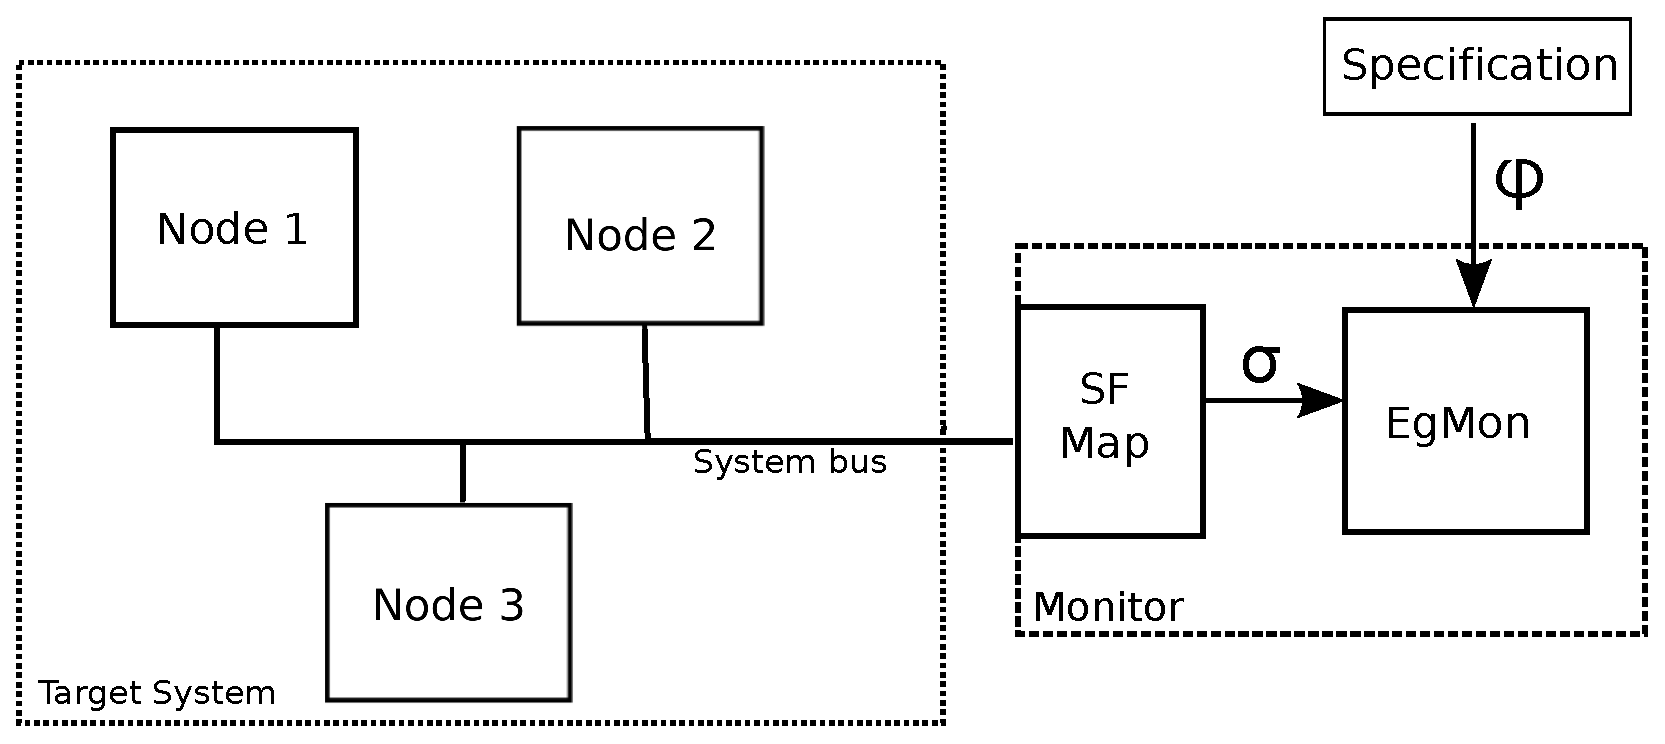
\includegraphics[width=4.5in]{img/newArch}
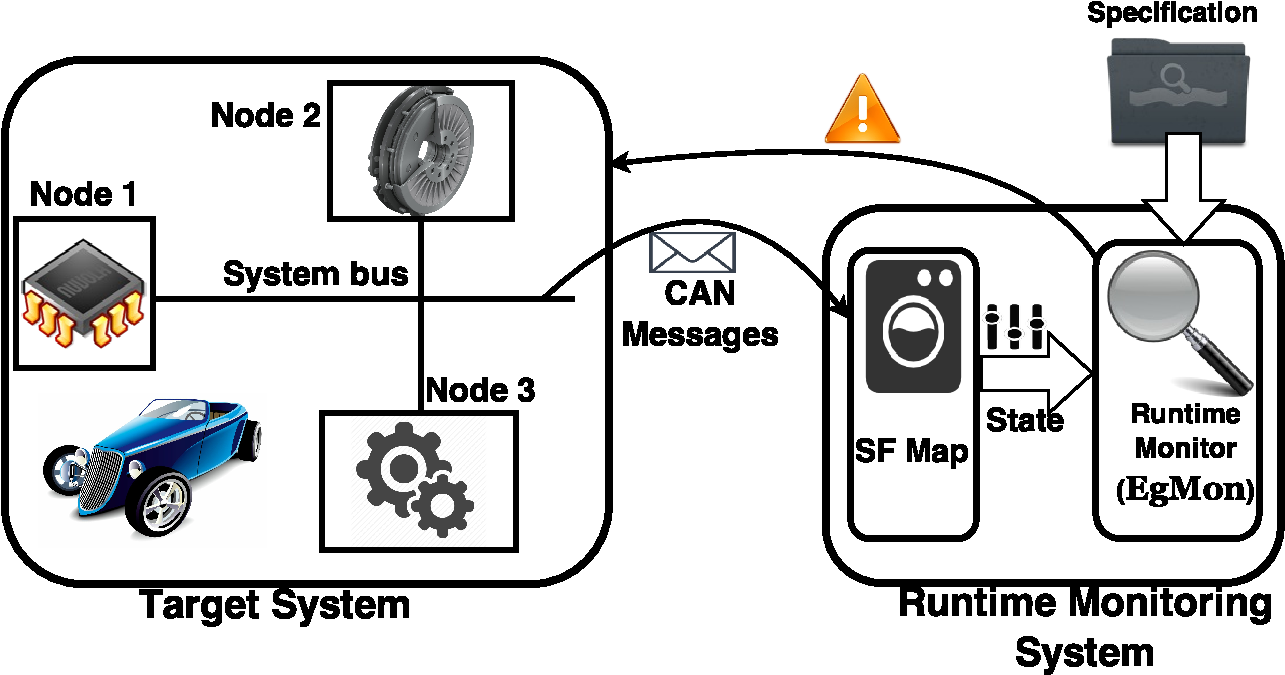
\includegraphics[scale=0.5]{img/ARV-main.pdf}
\caption{External monitor architecture outline \label{fig:architecture}}
\end{figure}


\subsection{Architecture Outline}
An outline of our monitor architecture is shown in Figure \ref{fig:architecture}. 
The monitor is connected to the target system as an additional passive node on its broadcast bus. 
% sfmap paragraph
Different systems have varying specification needs which can not always be easily met within a formal specification language. 
In order to provide flexibility to map system state onto the formal specification language (in our case, in propositions) we provide a \sfmap interface which defines the mapping between the observed system state and the monitored specification. 
This type of interface is common in monitors for real systems, including MaC's filters \cite{Kim2004} and the AP evaluation filter from \cite{Heffernan2014}.
%% 
The monitor's \sfmap generates the system trace by building the necessary propositions based on the observed bus traffic. 
This generated trace is provided to the monitoring algorithm which checks it against the given system specification, outputting whether the trace violated or satisfied the specification at each trace step (subject to delays waiting on future trace state).
%% took action controller out of arch picture so let's not mention it, could add it back in if we want...
%The algorithm's output is sent to an action controller which can perform the desired response to any specification violations, such as logging the violations or triggering a recovery action.

%\begin{figure}[!t]
%%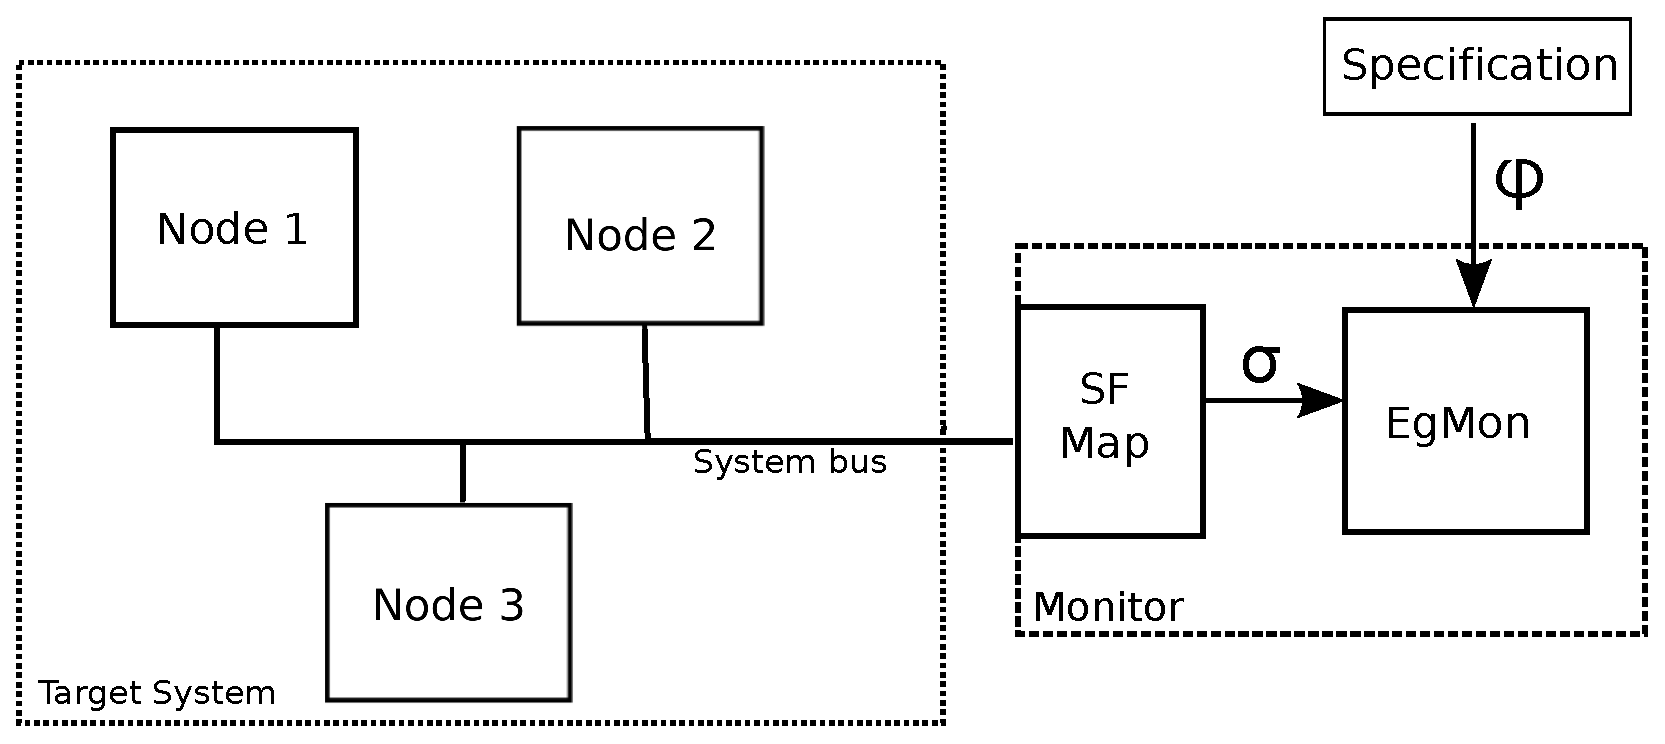
\includegraphics[width=4.5in]{img/newArch}
%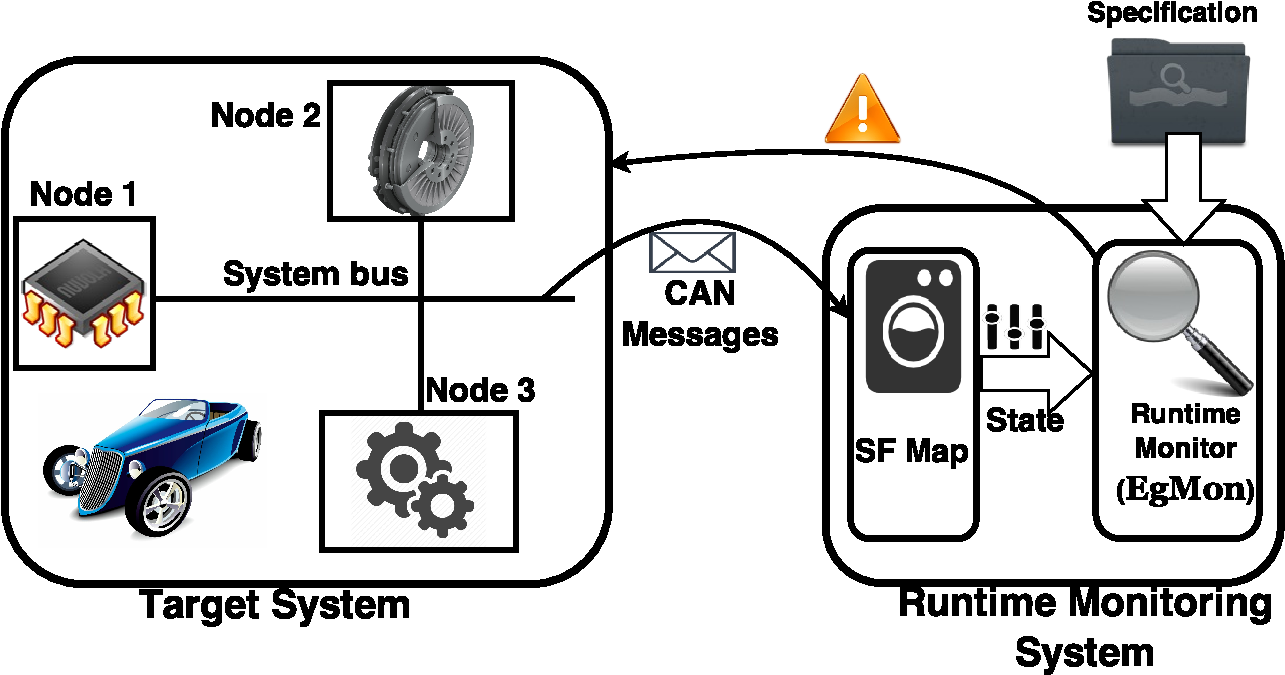
\includegraphics[scale=0.5]{img/ARV-main.pdf}
%\caption{External monitor architecture outline \label{fig:architecture}}
%\end{figure}

This architecture separates the lower-level system dependent configuration from the high-level system specification in a way similar to the architecture used in MaC \cite{Kim2004}.
%This architecture separates the system-independent formal aspects of the monitor from the system-dependent components including the system interface and action controller. 
%By utilizing a semi-formal interface, we can separate the formal aspects of the monitor, which are completely independent from the target system, from the more practical pieces: the monitor interfaces and their configurations, which are system dependent. 
This allows us to utilize a core formal monitoring algorithm and framework with any system where an \sfmap can be used to create a system trace.
Separating the system dependent and system-independent aspects of the monitor also lets the high level system requirements be somewhat abstracted away from the implementation. 
This helps keep the monitoring specification matched closer to the system requirements documentation which usually does not include low-level implementation details. 
This also helps the monitor handle changes in the target system. If the system changes in a way that affects the monitoring-relevant messages, only the \sfmap configuration needs to be updated, rather than the monitor itself.
%This is a similar situation to the two-level specifications used in the MaC framework \cite{Kim2004}.


%%%%% Algorithm section

\section{Monitoring Algorithm}
%% Why our algorithm...
%%% MTL due to explicit time restrictions
%%% need real-time finite trace checking

%In order to
For checking whether the given ARV system  adheres to its specification,
%distributed embedded systems
we need an algorithm which %can %continuously
incrementally checks explicit time specifications (\ie, propositional metric-time temporal logic~\cite{Koymans1990})
over finite, timed system traces (Every trace position of a \emph{timed trace} has an explicit time associated with it).
This has led to our algorithm \monitor which is an iterative monitoring algorithm based on formula rewriting and summarizing the relevant history of the trace
in \emph{history-structures}. To detect violations early, \monitor, eagerly checks whether it can reduce subformulas of the original formula to boolean value
%either true/false
using formula simplifications (\eg, $a\wedge \mathit{false} \equiv \mathit{false}$).
Many of the existing algorithms for evaluating formulas like $\eventually_{[l,h]} a \vee b$
(read, either $b$ is true or sometimes in the future $a$ is true such that the time difference
between the evaluation state and the future state in which $a$ is true, $t_d$, is within the
bound $[l,h]$) wait enough time so that $\eventually_{[l,h]} a$ can be fully evaluated.
\monitor however tries to eagerly evaluate both $\eventually_{[l,h]} a$ and $b$ and see
whether it can reduce the whole formula to boolean value.
For another eagerness checking example,
let us assume we are checking the property $a\until_{[l, h]}b$ (read, the formula is true at trace position $i$ if there is a trace position
$j$ in which $b$ holds such that $j\geq i$ and the time difference between position $i$ and $j$ is in the range $[l,h]$
and for all trace positions $k$ such that $i\leq k < j$ the formula $a$ holds) at trace position $i$.
While monitoring if we can find a trace position $k > i$ for which $b$ and $a$ are both false then we can evaluate the formula to be
false without waiting for a trace position in which $b$ is true. Nesting of  temporal formulas can make the eager check nontrivial.
We want to emphasize that \monitor optimistically
checks for violations and hence we could possible have a trace in which each formula can only be evaluated in
the last possible trace position then our algorithm will behave in the exact same way as the non-eager
algorithms modulo the extra computation for eager checking.
%either true or false.
%
%To constantly check that the target system is adhering to its specification, we must constantly check the specification against the current system trace. To constantly check the system efficiently, \monitor is an iterative algorithm, performing additional checking as each new trace step arrives.

\subsection{Specification Logic}
Many safety specification rules for ARV-like systems require explicit time bounds to ensure timely behavior,
so a specification language with explicit time bounds is important.
For instance,
%Examples of rules that utilize explicit time bounds include: %
``\natlangrule{cruise control shall disengage for 250ms within 500ms of the brake pedal being depressed}''
($\pred{brakeDepress} \rightarrow \eventually_{[0, 500]} \henceforth_{[0,250]} \neg \pred{CruiseEng}$).
%,
%\natlangrule{the cruise control mode cannot transition directly from Off to Engaged within 250ms} ($\neg (\pred{CruiseEngaged} \wedge \yesterday_{[0,250]} \pred{CruiseOff})$),
%and \natlangrule{the vehicle should not be within 1m of the current lane edge for 1s while lane centering is enabled} ($\neg \historically_{[0, 1000]}(\pred{LaneCentering} \wedge \pred{distToLaneEdgeLT1m})$).
Our safety specification language for the ARV system, which we call \planguage, is a future-bounded,
discrete time, propositional metric temporal logic (MTL \cite{Koymans1990}).
%%past temporal operators may have infinite bounds but
%where
%future temporal operators must have finite bounds.
%(\ie, $l$ and $h$ are both finite).
The syntax of \planguage is as follows:

\vspace*{1pt}
\(
\begin{array}{ccc}
\policy & ::=  & \true \mid \pred{p} \mid \neg \policy \mid \policy_1\vee \policy_2\mid
\policy_1\since_{\interval}\policy_2 \mid \policy_1\until_{\interval}\policy_2\mid\yesterday_{\interval}\policy\mid \tomorrow_{\interval}\policy
\end{array}
\) \\
\textit{Syntax.}
\planguage has logical true (\ie, \true),
 propositions $\pred{p}$, logical connectives (\ie, $\neg, \vee$),
past temporal operators \emph{since} and \emph{yesterday} $(\since, \yesterday)$,
and future temporal operators \emph{until} and \emph{next} $(\until, \tomorrow)$.
Other temporal operators (\ie, \once,\historically,\eventually,\henceforth) can be easily derived
from the ones above.
There is a bound $\mathbb{I}$ of form $[l,h]$ ($l\leq h$ and $l,h\in\mathbb{N}\cup\infty$)
associated with each temporal operator.
Note that the bound  $[l,h]$ associated with the future temporal operators must be finite.
Specification propositions \pred{p} come from a finite set of propositions provided in
the system trace by the \sfmap.
These propositions are derived from the observable system state and represent specific system properties, for instance,
proposition $\pred{speedLT40mph}$ could describe whether the vehicle speed is less than 40mph.
We use \policy, $\phi$, $\alpha$, and $\beta$ (possibly with subscripts) to denote valid \planguage formulas.
%


\textit{Semantics. }
\planguage formulas are interpreted over time-stamped \emph{traces}. A trace $\sigma$ is a sequence of states, each of which maps all propositions in \sfmap, to either \true or \false. We denote the $i^{th}$ position of the trace with $\sigma_i$ where $i\in\mathbb{N}$. Moreover, each $\sigma_i$ has an associated time stamp denoted by $\tau_i$ where $\tau_i\in\mathbb{N}$.
We denote the sequence of time stamps with $\tau$. For all $i, j\in\mathbb{N}$ such that $i < j$, we require $\tau_i < \tau_j$. For a given trace $\sigma$ and time stamp sequence $\tau$, we write $\sigma, \tau, i\models\policy$ to denote that the formula \policy is true with respect to the $i^{th}$ position of $\sigma$ and $\tau$.
The semantics of \planguage future bounded MTL is standard, see for instance, \cite{Basin2008}.
Each  property \policy has an implicit unbounded \henceforth future operator ($\henceforth\policy$ signifies that
\policy is true in all future trace positions including the current trace position) at the top-level and we handle it by
checking whether \policy is true in each trace position.
% is evaluated over the trace at every trace step (\ie, there is an implicit unbounded always over all top-level specification formulas.

\[
\tempSub(\policy) = \begin{cases}
\emptyset & \mbox{ if } \policy \equiv p\\
\{\alpha\} \cup \{\beta\} \cup \tempSub(\alpha) \cup \tempSub(\beta) & \mbox{ if } \policy\equiv\alpha\until_\mathbb{I}\beta|\alpha\since_\mathbb{I}\beta\\
\tempSub(\alpha) \cup \tempSub(\beta) & \mbox{ if } \policy\equiv\alpha\vee\beta\\
\tempSub(\alpha) & \mbox{ if }\policy\equiv\neg\alpha
\end{cases}
\]
% \textit{Auxiliary notions.}
We now introduce the readers with some auxiliary notions which will be
necessary to understand our algorithm \monitor. We first define ``\emph{residual formulas}'' or, just ``\emph{residues}''.
Given a formula \policy, we call another formula \policyv as \policy's residual, if we obtain \policyv after evaluating \policy with respect to the current information of the trace.
Note that a formula residue might not be a truth value if the formula could not conclusively be reduced given the current trace state (e.g, if future state is required to determine the truth value).
A residue $r^j_{\policy}$ is a tagged pair $\rpt{j}{\policyv}{\policy}$ where $j$ is a position in the trace in which we intend to evaluate $\policy$ (the original formula) and $\policyv$ is the current residual formula. We use these residues to efficiently hold trace history for evaluating temporal formulas.
%
%Our monitoring algorithm utilizes \emph{residues}, which are partially reduced (\ie, rewritten) policy formulas representing the remaining portion of a formula which could not be fully evaluated given the current trace. A residue $r^j_{\policy}$ is a tagged pair $\rpt{j}{\policyv}{\policy}$ where $j$ is a position in the trace, $\policy$ is the original residue formula and $\policyv$ is the residual formula. We use these residues to efficiently hold policy history for future time formulas which cannot be evaluated due to incomplete information.
The next notion we introduce is of ``\emph{wait delay}''. It is a function \wdelay that takes as input a formula \policy and
$\wdelay(\policy)$ returns
%Policy formulas have a wait delay $\wdelay(\policy)$ which defines
an upper bound on the time one has to wait before they can evaluate \policy with certainty.
%duration necessary to guarantee complete information to evaluate the formula.
For past- and present-time formulas \policyv, $\wdelay(\policyv)=0$.
%,
%as \policyv can be evaluated currently.
%since all trace steps necessary to evaluate them have already been seen by the monitor.
Future time formulas have a delay based on the interval of the future operator
(\eg, $\wdelay(\LTLdiamond_{[0,3]} \pred{p}) = 3$). The length of a formula $\policy$, denoted $|\policy|$, returns the total number of subformulas of \policy.
%, (\ie, the number of nodes in the policy AST).
The function \tempSub takes as input a formula \policy, and returns all the temporal subformulas \policyv of \policy and strict subformulas of \policyv.



%To evaluate an \planguage formula \policy, we may need to save a limited amount of
%past evaluation results for some temporal subformulas of \policy. We call this the \emph{history}.
%%history state of child policies of temporal subformula within a policy.
%For example, given the formula $\pred{ACCCancelReq} \rightarrow \eventually_{\interval} \pred{ACCOff} \vee (\pred{ACCOn} \since_{\interval} \pred{ACCCancelReq})$, $\pred{ACCOff}$ is a child policy of the temporal formula $\eventually_{\interval} \pred{ACCOff}$ and $\pred{ACCOn}$ and $\pred{ACCCancelReq}$ are children of the temporal formula $\pred{ACCOn} \since_{\interval} \pred{ACCCancelReq}$.
%The monitor must store some history of these child policies in order to evaluate the parent policy.
%The operation $\tempSub(\varphi)$ identifies all the children of temporal subformula of a policy $\varphi$.
%%% might want to do a more abstract example to show recursiveness
%%That is, for $\alpha\, \mathcal{U}_{[l,h]}\, \beta$ we need to save the history of $\alpha$ and $\beta$ (and if either of those are also a temporal formula then we need their history as well).


%% maybe need formula length, storage delay, simplify\dots


\subsection{\monitor Algorithm}
Our runtime monitoring algorithm \monitor takes as input an
\planguage formula $\policy$ and monitors a growing trace,
building history structures and reporting the specification violations
as soon as they are detected. We summarize the relevant algorithm functions below:

\begin{description}
\item[$\monitor{}(\policy)$] is the top-level function.
\item[$\reduce(\sigma_i, \tau_i, \histSt{i}, \rpt{i}{\policy}{\policy})$] reduces the given residue based on the current state $(\sigma_i,\tau_i)$ and the history $\histSt{i}$.
\item[$\tempSub(\policy)$] identifies the subformulas which require a history structure to evaluate the formula $\policy$.
\item[$\incrS(\histst{i-1}, \histSt{i}, \sigma_i, \tau_i, i)$] updates the history structure $\histst{i-1}$ to step $i$ given the current trace and history state.
\end{description}




\textbf{Top-level monitoring algorithm.}
The top-level monitoring algorithm \monitor is a sampling-based periodic monitor which uses history structures to store trace state for evaluating temporal subformulas.
\emph{History structures} are lists of residues along with past-time markers for evaluating infinite past-time formulas.
The algorithm checks the given formula $\policy$ periodically at every trace sample step.
When the fomula cannot be decided at a given step (\eg, it requires future state to evaluate), the remaining formula residue is saved in a history structure for evaluation in future steps when the state will be available.
The history structure for formula $\policyv$ at trace step $i$ is denoted $\histst[\policyv]{i}$.
We use $\histSt[\policy]{i}$ to denote the set of history structures for all temporal subformula of $\policy$, \ie,
$\histSt[\policy]{i} = \bigcup_{\policyv \in \tempSub(\policy)} \histst[\policyv]{i}$.


The high level algorithm \monitor is shown in Figure \ref{fig:algorithm}.
%
First, all the necessary history structures $\histst[\policyv]{ }$ are identified using $\tempSub(\policy)$ and initialized.
Once these structures are identified, the monitoring loop begins.
%
In each step, all the history structures are updated with the new trace step.
This is done in increasing formula size since larger formula can depend on the history of smaller formula (which may be their subformula).
%
Each structure is updated using $\incrS(\histst[\policyv]{i-1},\histSt[\policyv]{i}, \sigma_i, \tau_i, i)$ which adds a residue for the current trace step to the structure and reduces all the contained residues with the new step state.
Then, the same procedure is performed for the top level formula that is being monitored -- the formula's structure is updated with $\incrS(\histst{i-1},\histSt{i},\sigma_i,\tau_i, i)$.
Once updated, this structure contains the evaluation of the top-level formula. The algorithm reports any identified formula violations (\ie, any $\false$ residues) before continuing to the next trace step.
%
We note that due to the recursive nature of the monitoring algorithm, the top-level formula is treated exactly the same as any temporal subformula would be (which follows from the fact that the top-level formula contains an implicit \emph{always} $\henceforth$).
The history structure updates for the top-level formula are separated in the algorithm description for clarity only.
The only difference between the top-level formula and other temporal subformula is that violations are reported for the top-level formula.




% \begin{figure}
% \begin{align}
% \tempSub(\phi) &= \emptyset &\text{if } \phi \equiv p \\
% 			   &= \{\alpha\} \cup \{\beta\} \cup \tempSub(\alpha) \cup \tempSub(\beta) &\text{if } \phi \equiv \alpha \until \beta \\
% 			   &				&\text{or } \phi \equiv \alpha \since \beta \\
% 			   &= \tempSub(\alpha) \cup \tempSub(\beta) &\text{if } \phi \equiv \alpha \vee \beta \\
% 			   &= \tempSub(\alpha) &\text{if } \phi \equiv \neg \alpha \\
% \end{align}
% \end{figure}

\begin{figure}[t]
\begin{algorithmic}[1]
%\STATE Recognize formulas for which we build structures
\STATE For all recognized formulas $\policyv \in \tempSub(\policy)$: $\histst[\policyv]{-1} \leftarrow \emptyset$
\STATE $i \leftarrow 0$
\LOOP
\STATE Obtain next trace step $(\sigma_i, \tau_i)$
\FOR{every $\policyv \in \tempSub(\policy)$ in increasing size}
	\STATE $\histst[\policyv]{i} \leftarrow \incrS(\histst[\policyv]{i-1}, \histSt[\policyv]{i}, \sigma_i, \tau_i, i)$
\ENDFOR
\STATE $\histst{i} \leftarrow \incrS(\histst{i-1}, \histSt{i}, \sigma_i, \tau_i, i)$
%\FOR{all $\rp{j}{\bot} \in S^i_{\varphi}$}
\FOR{all $\rp{j}{\false} \in \histst{i}$}
\STATE \texttt{Report violation on $\sigma$ at position $j$}
\ENDFOR
\STATE $i \leftarrow i + 1$
\ENDLOOP
\end{algorithmic}
\caption{\monitor Algorithm}\label{fig:algorithm}
\end{figure}

\textbf{Reducing Residues.}
\monitor works primarily by reducing formula residues down to truth values. Residues are reduced by the $\reduce(\sigma_i, \tau_i, \histSt{i}, \rpt{j}{\policyv}{\policy})$ function, which uses the current state ($\sigma_i,\tau_i$) and the stored history in $\histSt{i}$ to rewrite the formula $\policyv$ to a reduced form, either a truth value or a new formula which will evaluate to the same truth value as the original. For past or present-time formulas, $\reduce()$ is able to return a truth value residue since all the necessary information to decide the formula is available in the history and current state. Future-time policies may be fully-reducible if enough state information is available. If a future-time formula cannot be reduced to a truth value, it is returned as a reduced (potentially unchanged) residue.

% reduce for until
For residues whose formula is an \emph{until} formula $\alpha \until_{[l,h]} \beta$, the history structures $\histst[\alpha]{i}$ and $\histst[\beta]{i}$ are used to reduce the formula.
If the formula can be evaluated conclusively then the truth value is returned, otherwise the residue is returned unchanged.
Figure \ref{fig:until} shows the reduction algorithm for \emph{until} temporal formula. Reducing \emph{since} formulas is essentially the same except with reversed minimum/maximums and past time bounds.

%%% TAU UNTIL
\begin{figure}
\small
\begin{align*}
\mathbf{reduce}(\sigma_i,\tau, i,\mathbb{S}^i_{\alpha\, \mathcal{U}_{[l,h]}\, \beta} ,\rp{j}{\alpha\, \mathcal{U}_{[l,h]}\, \beta}) = \left\{
\begin{aligned}
&\text{let } a_a \leftarrow min(\{k | \tau_j \leq \tau_k \leq \tau_j+h  \wedge \rp{k}{\bot} \in S^i_\alpha \},i) \\
% a_u
%& a_u \leftarrow max({k| \tau_j \leq \tau_k \leq \tau_j+h \wedge \rp{k}{\alpha'} \in S^i_\alpha \wedge \alpha' \not\equiv \top},i) \\
& a_u \leftarrow max(\{k| \tau_k \in [\tau_j,\tau_j+h] \\
& \quad \quad \quad \wedge \forall k' \in [j,k-1].(\rp{k'}{\alpha'} \in S^i_\alpha \wedge \alpha' \equiv \top\},i) \\
% b_a
& b_a \leftarrow min(\{k | \tau_j+l \leq \tau_k \leq \tau_j+h \wedge \rp{k}{\beta'} \in S^i_\beta \wedge \beta' \neq \bot\}) \\
% b_t
&b_t \leftarrow min(\{k | \tau_j+l \leq \tau_k \leq \tau_j+h \wedge \rp{k}{\top} \in S^i_{\beta} \}) \\
% b_n
&b_n \leftarrow \top \text{ if } (\tau_i - \tau_j \geq \wdelay(\psi)) \\
& \quad \quad \quad \wedge \forall k.(\tau_j+l \leq \tau_k \leq \tau_j+h). \rp{k}{\bot} \in S^i_{\beta} \\
&\text{if } b_t \neq \emptyset \wedge a_u \geq b_t \\
& \quad\mathbf{return} \rp{j}{\top} \\
&\text{else if } (b_a \neq \emptyset \wedge a_a < b_a) \text{ or } b_n = \top\\ & \quad\mathbf{return} \rp{j}{\bot} \\
&\text{else} \\
& \quad\mathbf{return} \rp{j}{\alpha\, \mathcal{U}_{[l,h]}\, \beta}
\end{aligned} \right. \\
\end{align*}
%\normalsize
\caption{Definition of \reduce for \emph{until} formulas \label{fig:until}}
\end{figure}

The \reduce function for $\emph{until}$ formulas uses marker values to evaluate the semantics of $\emph{until}$. \reduce calculates five marker values: $a_a$ is the earliest step within the time interval where $\alpha$ is known false. $a_u$ is the latest step within the interval that $\alpha \until_{[l,h]} \beta$ would be true if $\beta$ were true at that step. $b_a$ is the earliest step within the interval at which $\beta$ is not conclusively false, and $b_t$ is the earliest step within the interval at which $\beta$ is conclusively true. $b_n$ holds whether the current step $i$ is later than the wait delay and all $\beta$ values within the interval are false. With these marker variables, reduce can directly check the semantics of \emph{until}, and either return the correct value or the unchanged residue if the semantics are not conclusive with the current history. Reducing \emph{since} formulas works in the same way (using the same marker values) adjusted to past time intervals and utilizing the unbounded past time history values.


\textbf{Incrementing History Structures.}
To evaluate past and future-time policies, we must correctly store trace history which can be looked up during a residue reduction.
We store the trace history of a formula $\policyv$ in a history structure $\histst[\policyv]{}$.
This history structure contains a list of residues for the number of steps required to evaluate the top-level formula. History structures are incremented by the function
$\incrS(\histst[\policyv]{i-1}, \histSt[\policyv]{i}, \sigma_i, \tau_i, i) = (\bigcup_{r \in \histst[\policyv]{i-1}} \reduce(\sigma_i, \tau_i, \histst[\policyv]{i}, r)) \cup \reduce(\sigma_i, \tau_i, \histst[\policyv]{i}, \rp{i}{\policyv})$
%
This function takes the previous step's history structure $\histst[\policyv]{i-1}$ and the current state
%($\sigma_i,\tau_i$, and the updated smaller history structures $\histSt[\policyv]{i}$)
and performs two actions:
%\begin{enumerate}
	1) Adds a residue for the current step $i$ to $\histst[\policyv]{i-1}$ and
	2) Reduces all residues contained in $\histst[\policyv]{i-1}$ with the current state.
%\end{enumerate}
%Together, these two actions leave an updated history structure $\histst[\policyv]{i}$ which has updated history information for all the required steps.


\subsection{Algorithm Properties}
There are two important properties of \monitor which need to be shown. First, \emph{correctness} states that the algorithm's
results are correct.
That is, that if \monitor reports a property violation, the trace really did violate the property. Second, \emph{promptness}  requires that
the algorithm provide a decision for the given property in a timely fashion (\ie, with $t$ such that $t\leq \wdelay(\policy)$).
%at any given time $t$ within a finite bound, $\wdelay(\policy)$.
 Promptness precisely requires that the algorithm decides satisfaction of the given
property at trace position $i$ as soon as  there is another
trace position $j$ available such that $j\geq i$ and $\tau_j-\tau_i \geq \wdelay(\policy)$.
Note that it is possible to define a stronger notion of promptness, \emph{strong promptness}, which
ensures that the runtime monitor makes a judgement about the satisfaction of a property as soon as
it is possible to do so. In this discussion we however we only consider promptness.
%guaranteed to be possible to decide.
%
%Besides correctness guarantees, our algorithm is also \emph{eager}. An eager algorithm reports satisfaction as soon as the trace is an informative prefix \cite{Kupferman2001} for the policy.
%Many temporal policies can be evaluated before the promptness delay, providing early detection and extra time for recovery actions compared to other monitoring algorithms which wait until the promptness delay to ensure they can check the policy.
%
The following theorem states that \monitor is correct and prompt. It requires  the history structures $\histSt{i}$ to be consistent at $i$ analogous to the trace $\sigma,\tau$.
This means that the history structures contain correct history of the trace till step $i$. %The algorithm provides this consistency itself if run iteratively from step $0$.

\begin{theorem}[Correctness and Promptness of \monitor]
For all $i \in \mathbb{N}$, all formula $\varphi$, all time stamp sequences $\tau$ and all traces $\sigma$ it is the case that (1) if $\rp{j}{\false} \in \histst{i}$ then $\sigma, \tau, j \nvDash \policy$ and if $\rp{j}{\true} \in \histst{i}$ then $\sigma, \tau, j \vDash \policy$ (Correctness) and (2) if $\tau_i - \tau_j \geq \wdelay(\policy)$ then if $\sigma, \tau, j \nvDash \policy$ then $\rp{j}{\false} \in \histst{i}$ and if $\sigma, \tau, j \vDash \policy$ then $\rp{j}{\true} \in \histst{i}$ (Promptness)
.
\end{theorem}
\textit{Proof.} By  induction on the  formula $\policy$ and time step $i$. See \cite{Kane2015} \\

We now discuss the runtime complexity of \monitor while checking satisfaction of a property \policy. At any
most recent position of the trace, let us assume we have maximum $L$ positions in the current trace
for which \policy has not yet
been reduced to a boolean value.
Note that if the value of $\wdelay(\policy)$ is large $L$ can be as large as the current trace length we have seen so far.
Addtionally, for each temporal subformula $\phi_1\until\phi_2$ of \policy,
we build history structures that
keep track of segments of the trace positions for which $\phi_1$ is true. Let  assume
we have $S$ such segments that are relevant (relevant means they can possibly
influence the satisfaction of the remaining unreduced formulas).
Hence, the complexity of \monitor is
$\mathcal{O}(LM|\policy|)$.

%Theorem \ref{thm:eagerness} states that \monitor is eager.
%
%\begin{theorem}[Eagerness of \monitor]
%\label{thm:eagerness}
%For all $i \in \mathbb{N}$, all formula $\varphi$, all time stamp sequences $\tau$ and all traces $\sigma$ it is the case that (1) if $\sigma_0,\ldots,\sigma_i$ is an informative prefix then if $\sigma,\tau, i \vDash \policy$ then $\rpt{i}{\true}{\policy} \in \histst{i}$ and if $\sigma, \tau, i \nvDash \policy$ then $\rpt{i}{\false}{\policy} \in \histst{i}$.
%\end{theorem}
%\textit{Proof.} By mutual induction on the policy formula $\policy$ and time step $i$. See \cite{TechPaper}
%%%%%%%%%%%%%%%%%%%%%%%%%%% REWRITE LINE %%%%%%%%%%%%%%%%%%%%%
%%%%%%%%%%%%%%%%%%%%%%%%%%% REWRITE LINE %%%%%%%%%%%%%%%%%%%%%

%%% New implementation section 

\section{Monitor Implementation and Evaluation}

%% paragraph 1 -- goals
To evaluate the feasibility of our monitoring algorithm for safety-critical real-time systems we have built a real-time CAN monitor on an ARM Cortex-M4 development board. This allowed us to explore the necessary optimizations and features required to perform real-time checking of realistic safety policies.

%% paragraph 2 -- what we built

%% Embedded restrictions
Software for safety-critical embedded systems typically contains more strict design and programming model constraints than less critical software. Two important and common constraints for these systems are avoiding recursion and not using dynamic memory allocations. 
% dynamic memory alloc
Common safety-critical coding guidelines discourage or prohibit dynamic memory allocation to avoid memory leaks.
Because our specification language is bounded, we can avoid dynamic allocation in our \monitor implementation by statically allocating space for the maximum number of entries for our history structures and other temporary data structures.
% recursion
Recursion is also usually prohibited because it can be difficult to guarantee a maximum stack depth when using recursion. Although \monitor utilizes recursion extensively, we can implement \monitor using a traditional iterative traversal of the specification formulas instead.

\subsection{Hybrid Algorithm}
Our eager monitoring algorithm attempts to evaluate specification rules as soon as possible, but this requires checking trace properties which may not be fully reducible given the current trace. These unfinished formula reductions require extra computation time, and in practice the majority of the policy reductions performed by \monitor will be these eager reductions which may not fully reduce.

While early detection of violations can be useful, there are situations where eagerly checking an entire target specification may require more computation than is available from the monitor in a given period.

To enable the benefits of eager checking while avoiding the risks of losing real-time correctness, we have implemented a hybrid eager monitoring algorithm which performs non-eager (conservative) checking first and uses any spare time to eagerly check the remaining monitor residues.
%
Conservative \monitor monitoring is performed by only checking residues which are older than their formula delay, which guarantees that these residue will be reduced at their first evaluation.
%
Under our periodic sampling design, each step of conservative monitor only requires updating the history structures and checking a single residue (the oldest remaining one) for each specification policy.
%
This conservative check can be done quickly at each period, leaving any extra time until the next period for eager checking. This provides a conservative monitoring guarantee (\ie, the specification is checked within a known promptness delay) while also allowing the monitor to eagerly check as much of the specification as possible.

%As long as we know that the worst case execution time for message handing, incrementing the structures, and a single residue check is short enough to finish within a monitor period then we are guaranteed at least a conservatively correct and prompt output.

\begin{figure}[t]
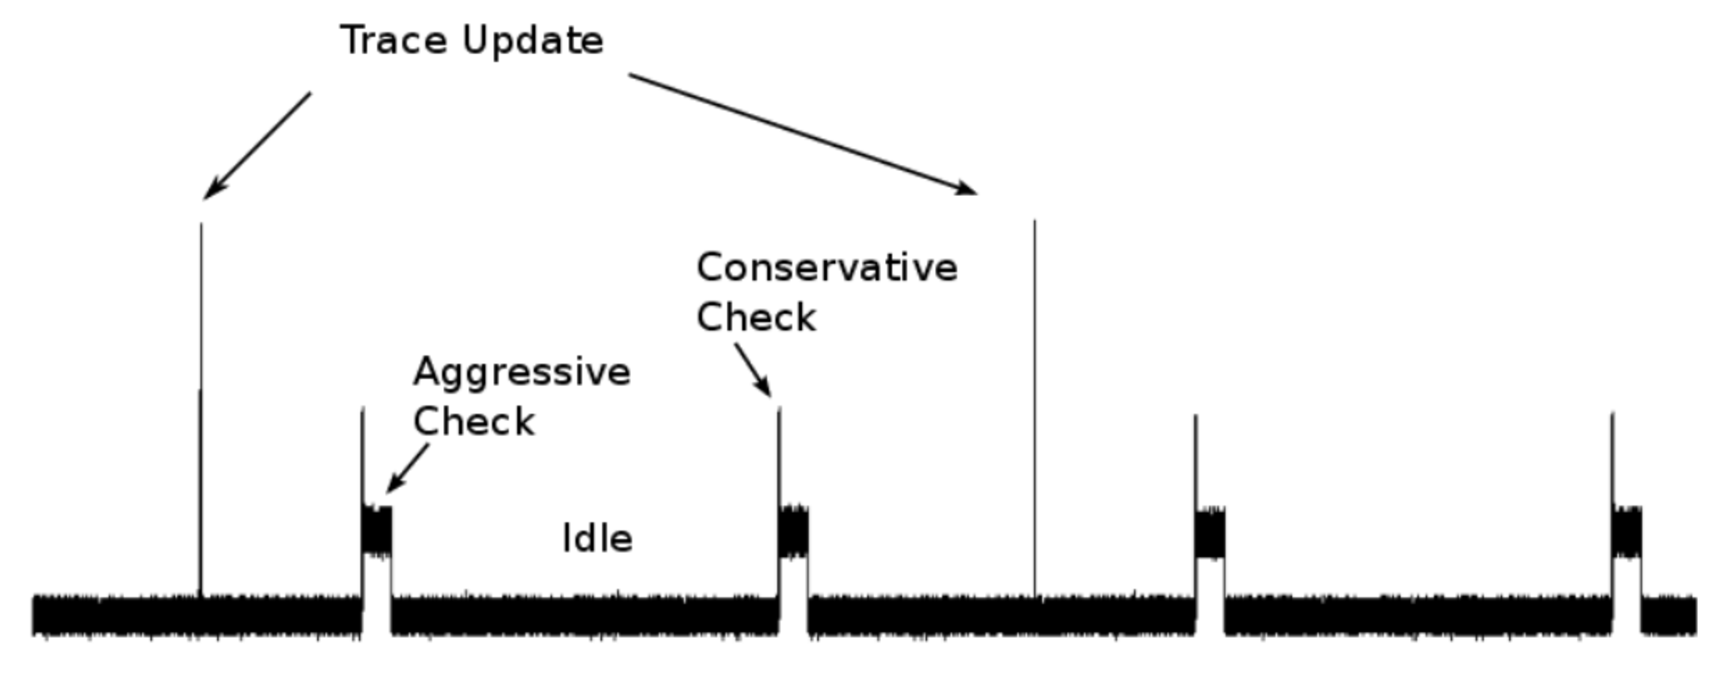
\includegraphics[width=4.5in]{img/scope_annotated_crop}
\caption{Oscilloscope capture of embedded monitor task execution \label{fig:arch:oscope}}
\end{figure}

We have implemented the hybrid monitoring algorithm in our embedded monitor. The monitor updates the history structures (shared between the conservative and eager checking) and performs a conservative check once every monitoring period. It then uses the idle time between periods to perform eager checking of any remaining unchecked specification properties.
%
Figure \ref{fig:arch:oscope} shows the execution of the embedded monitor instrumented to output the currently executing task to an oscilloscope. The residue checks run twice per trace update due to the monitor configuration used during the test, but this is not required for correct monitoring.
This task output was captured while monitoring the specification used in the case study (see Section \ref{sec:case_study} plus another 200 time-step \emph{eventually} rule which was never satisfied. 
%(guaranteeing an extra 200 eager residue checks every period). 
The rule never being satisfied means that at every step the monitor performed an eager check of all 200 residues for this rule at every step (i.e., since they were never satisfied, they could never be reduced early). 
Even with this excess computation there was still a large portion of extra idle time -- 23ms of the 25ms monitoring loop was spent idle. 
This shows the eager checking finished reasonably quickly and the monitor could handle much longer formula durations or more complex formulas before the execution time becomes bad enough to require the hybrid algorithm for correctness guarantees. 

\subsection{Case Study}
\label{sec:case_study}
This section reports our case study performing real-time monitoring of a CAN network for realistic safety properties. 
For this case study we have obtained CAN network logs from a series of robustness tests on the ARV which we have replayed on a test CAN bus for the monitor to check. 
This setup, %shown in Figure \ref{fig:replaySchem}, 
helps us show the feasibility of performing external bus monitoring on this class of system with real safety specifications.

%% removing, takes space and not that important
%\begin{figure}
%\centering
%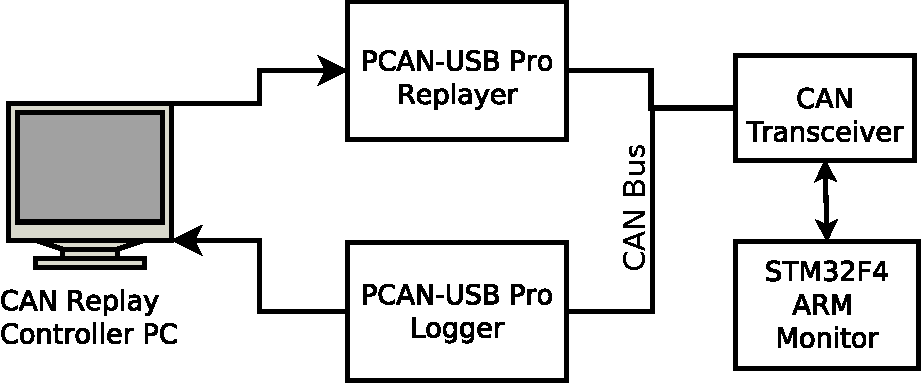
\includegraphics[width=3in]{img/replay_arch}
%\caption{CAN replay network setup \label{fig:replaySchem}}
%\end{figure}

%% paragraph 3 -- description of experiment 
%%% some of this is in para1, we should go over: specification, logs, etc
The logs contain both normal system operation as well as some operation under network-based robustness testing. During robustness testing, the testing framework can intercept targeted network messages on the bus and inject its own testing values. % could cite astaa here
A PC was connected to a PCAN-USB Pro \cite{PCAN-USBPro} device which provides a USB interface to two CAN connections. One CAN channel was used to replay the logs, while the other was used as a bus logger for analysis purposes.

%% paragraph 4 -- specification
Requirements documentation for this system was available, so we were able to build a monitoring specification based on actual system requirements.
The specification evaluated in the embedded monitor on the test logs are shown in Table \ref{tab:monspec}. This specification was derived from the system requirements based on the observable system state available in the testing logs. 



\begin{table}[t]
%\begin{tabular}{|p{3in}|l|}
\begin{tabular}{|l|p{4.5in}|}
\hline \multirow{2}{*}{Rule \#} & Informal Rule \\ & MTL \\
\hline \multirow{2}{*}{0} & A feature heartbeat will be sent within every 500ms \\
& $\pred{HeartbeatOn} \rightarrow \LTLdiamond_{[0,500ms]} \pred{HeartBeat}$ \\
\hline \multirow{2}{*}{1} & The interface component heartbeat counter is correct \\
& $\pred{HeartbeatOn} \rightarrow \pred{HeartbeatCounterOk}$ \\
\hline \multirow{2}{*}{2} & The vehicle shall not transition from manual mode to autonomous mode \\
&  $\neg ((\LTLcircleminus_{[0,25ms]} \pred{IntManualState}) \wedge \pred{IntAutoStat})$\\
\hline \multirow{2}{*}{3} & The vehicle controller shall not command a transition from manual mode to autonomous mode \\
& $\neg ((\LTLcircleminus_{[0,25ms]} \pred{VehManualModeCmd}) \wedge \pred{VehAutoModeCmd})$\\
\hline \multirow{2}{*}{4} & The vehicle shall not transition from system off mode to autonomous mode \\ 
&  $\neg ((\LTLcircleminus_{[0,25ms]} \pred{IntSDState}) \wedge \pred{IntAutoStat})$\\
\hline \multirow{2}{*}{5} & The vehicle controller shall not command a transition from system off mode to autonomous mode \\
& $\neg ((\LTLcircleminus_{[0,25ms]} \pred{VehSDModeCmd}) \wedge \pred{VehAutoModeCmd})$\\
% warn was at 200ms
\hline
\end{tabular}
\caption{Case study monitoring specification \label{tab:monspec}}
\end{table}

Rule \#0 is a heartbeat detection which ensures that the interface component is still running (essentially a watchdog message). Rule \#1 is a second component of this check. The system's heartbeat message contains a single heartbeat status bit which we checked directly in Rule \#0, but the message also has a rolling counter field. We use the \sfmap to ensure that this counter is incrementing correctly and output this check as the $\pred{HeartbeakOk}$ predicate which is checked in Rule \#1.
We also checked for illegal state transitions. Rules \#2 through \#5 check both for illegal transition commands from the vehicle controller and actual illegal state transitions in the interface component.

%% move hybrid algorithm explanation here maybe?

\subsection{Monitoring Results}
Monitoring the test logs with the above specification resulted in identifying two real violations as well as some false positive violation detections caused by the testing infrastructure.
%
% covering all three possible violation types. One was a false positive
Three different types of heartbeat violations were identified after inspecting the monitor results, some actual violations and some false-positives caused by the testing infrastructure. We also identified infrastructure-caused false-positive violations of the transition rules.

\begin{figure}[t]
		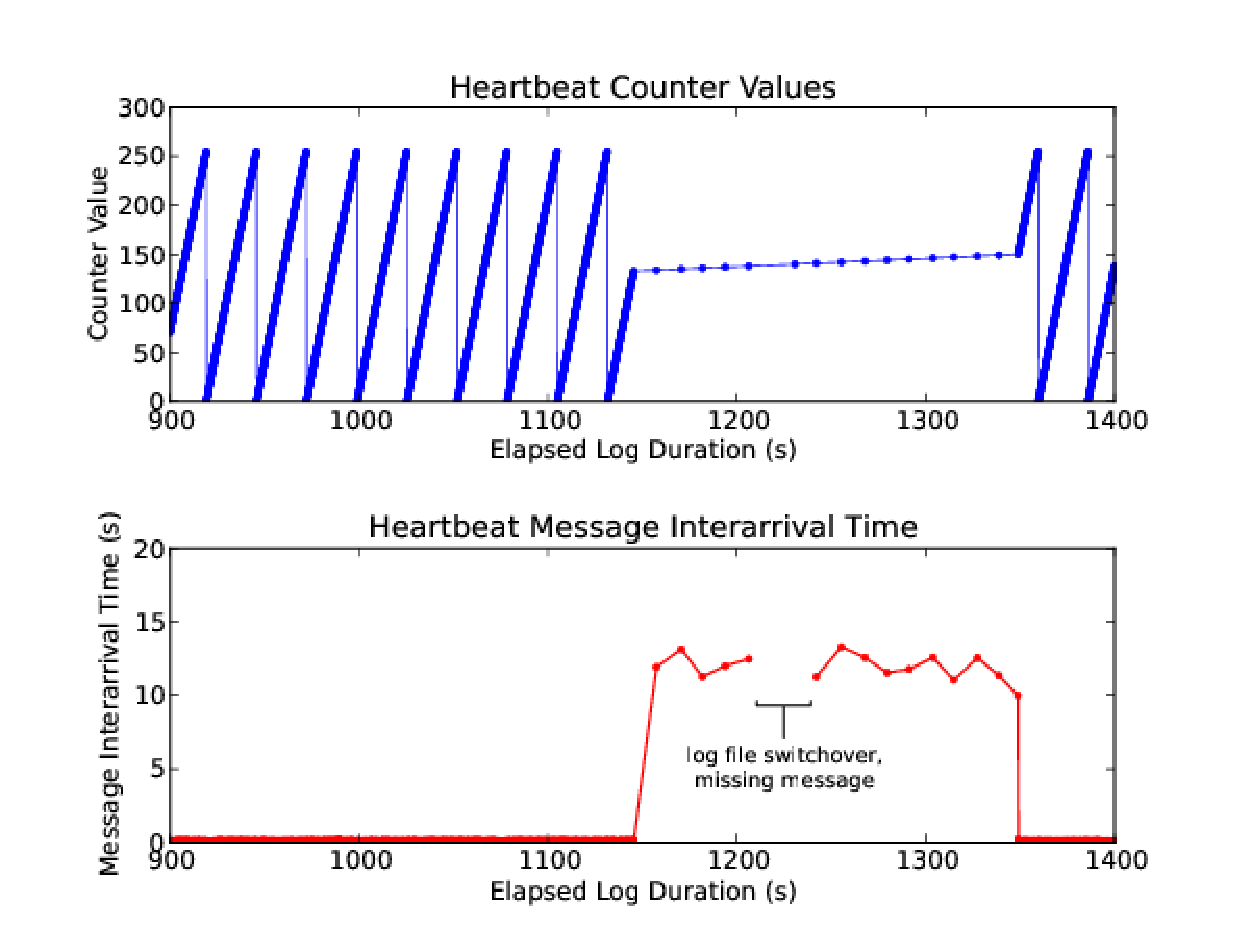
\includegraphics[width=4.5in]{img/hb1}
		\caption{Heartbeat counter values over time}
		\label{fig:hb_arrival}
\end{figure}

\paragraph{Specification violations.}
% missing hb message
The first violation is a late heartbeat message. In one of the robustness testing logs the heartbeat message was not sent on time, which is clearly a heartbeat violation. Figure \ref{fig:hb_arrival} shows the heartbeat counter values and the inter-arrival time of the heartbeat messages over time for this violation. We can see here that the heartbeat counter did in fact increment in a valid way, just too slowly. 
% bad status
The second violation is on-time heartbeat status message but the heartbeat status field is 0. 
We do not know from the available documentation whether a bad status in an on-time message with a good counter is valid or not. So without more information we cannot tell whether these violations are false positives or not. This is worthy of further investigation.


\begin{figure}[t]
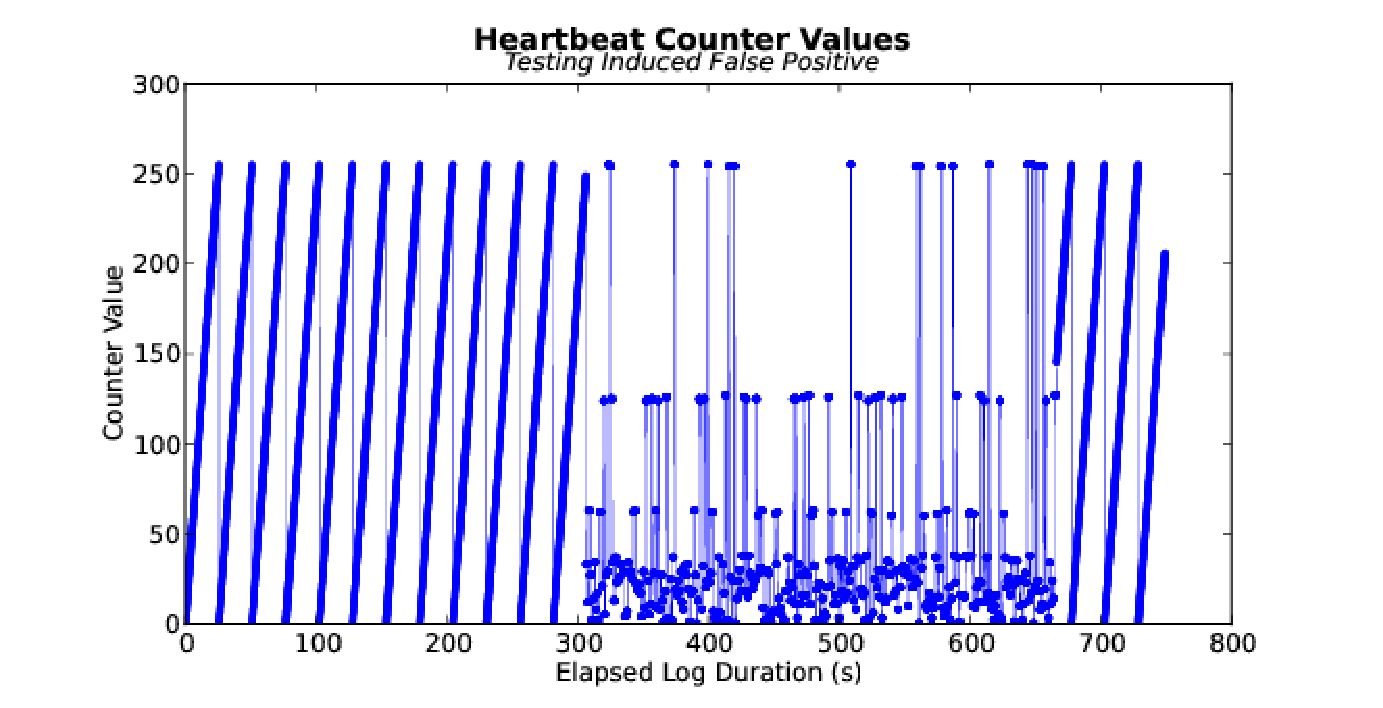
\includegraphics[width=4.5in]{img/hb2}
\caption{Bad heartbeat counter values \label{fig:hb_badcounter}}
\end{figure}

\paragraph{False-positive violations.}
% bad counter
The last type of heartbeat violation is a bad counter. 
We have defined a good counter as one which increments by one every message up to its maximum (255 in this case) before wrapping back to zero.
Every consecutive heartbeat status message must have an incremented heartbeat counter or a violation will be triggered. Figure \ref{fig:hb_badcounter} shows the counter value history for one of the traces with a heartbeat violation caused by a bad counter value.
%
%@EDIT describe robustness testing, define these false positives like the talk?
Further inspection of this violation showed that the bad counter values were sent by the testing framework rather than the actual system. In this case, the network traffic the monitor is seeing is not real system state but actually it is messages being injected by the testing framework. This is not a real violation (since the violating state is not the actual system state), and so we consider this a false positive violation.



The monitor also reported violations of the legal transition rules, but these, similar to the heartbeat counter violation, also turned out to be false positives triggered by message injections by the robustness testing harness. Since the monitor checks network state, if we perform testing that directly affects the values seen on the network (such as injection/interception of network messages) we may detect violations which are created by the testing framework rather than the system. 
Information about the test configurations can be used to filter out these types of false positives which arise from test-controlled state.
This type of filtering can be automated if the test information can be input to the monitor, either directly on the network (e.g., adding a message value to injected messages) or through a side-channel (i.e., building a testing-aware monitor).

%%%% Case study section


\section{Case Study}
\label{sec:case_study}
%% paragraph 1 -- experimental environment
This section reports our case study performing real-time monitoring of a CAN network for realistic safety properties. We have implemented the \monitor algorithm on a low cost ARM-Cortex M4 development board which can be used to monitor CAN networks. For this case study we have obtained CAN network logs from a series of robustness tests on an autonomous research vehicle which we have replayed on a test CAN bus for the monitor to check. This setup is shown in Figure \ref{fig:replaySchem}.

\begin{figure}
\centering
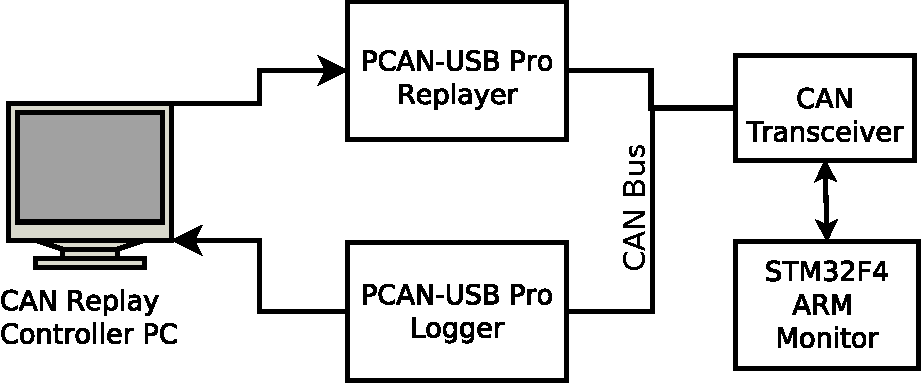
\includegraphics[width=3in]{img/replay_arch}
\caption{CAN replay network setup \label{fig:replaySchem}}
\end{figure}

%% paragraph 2 -- experiment goal
We wish to use the CAN monitor to check a realistic set of safety policies over a real network trace. From this, we can see the feasibility of performing external bus monitoring for these types of systems.

%% paragraph 3 -- description of experiment 
%%% some of this is in para1, we should go over: specification, logs, etc
The logs contain both normal operation as well as some operation under network-based robustness testing. During robustness testing, the testing framework can hijack targeted network messages on the bus to inject testing values. % could cite astaa here
A PC was connected to a PCAN-USB Pro \cite{PCAN-USBPro} device which provides a USB interface to two CAN connections. One CAN channel was used as the log replayer, while the other was used as a bus logger for analysis purposes.

%% paragraph 4 -- specification
Requirements documentation for this system was available, so we were able to build a monitoring specification based on actual system requirements.
The specification evaluated in the embedded monitor on the test logs are shown in Table \ref{tab:monspec}. This specification was derived from the system requirements based on the observable system state available in the testing logs. 


Rule \#0 is a heartbeat detection which ensures that the interface component is still running (essentially a watchdog message). Rule \#1 is a second component of this check. The system's heartbeat message contains a single heartbeat status bit which we checked directly in Rule \#0, but the message also has a rolling counter field. We use the system interface to ensure that this counter is correct, and check the system interface's output ($\pred{HeartbeatOk}$) in Rule \#1.
We also checked for illegal state transitions. Rules \#2 through \#5 check both for illegal transition commands and actual illegal state transitions.

\begin{table}
%\begin{tabular}{|p{3in}|l|}
\begin{tabular}{|l|p{4.5in}|}
\hline \multirow{2}{*}{Rule \#} & Informal Rule \\ & BMTL \\
\hline \multirow{2}{*}{0} & A feature heartbeat shall be received every 500ms \\
& $\pred{HeartbeatOn} \rightarrow \lozenge_{[0,500ms]} \pred{HeartBeat}$ \\
\hline \multirow{2}{*}{1} & The interface component heartbeat counter is correct \\
& $\pred{HeartbeatOn} \rightarrow \pred{HeartbeatCounterOk}$ \\
\hline \multirow{2}{*}{2} & The vehicle shall not transition from manual mode to autonomous mode \\
&  $\neg ((\blacksquare_{[1,1]} \pred{IntManualState}) \wedge \pred{IntAutoStat})$\\
\hline \multirow{2}{*}{3} & The vehicle controller shall not command a transition from manual mode to autonomous mode \\
& $\neg ((\blacksquare_{[1,1]} \pred{VehManualModeCmd}) \wedge \pred{VehAutoModeCmd})$\\
\hline \multirow{2}{*}{4} & The vehicle shall not transition from system off mode to autonomous mode \\ 
&  $\neg ((\blacksquare_{[1,1]} \pred{IntSDState}) \wedge \pred{IntAutoStat})$\\
\hline \multirow{2}{*}{5} & The vehicle controller shall not command a transition from system off mode to autonomous mode \\
& $\neg ((\blacksquare_{[1,1]} \pred{VehSDModeCmd}) \wedge \pred{VehAutoModeCmd})$\\
% warn was at 200ms
\hline
\end{tabular}
\caption{Case study monitoring specification \label{tab:monspec}}
\end{table}

%% move hybrid algorithm explanation here maybe?

\subsection{Monitoring Results}
Monitoring the test logs with the above specification resulted in identifying two real violations as well as some false positive violation detections caused by the testing infrastructure.

% covering all three possible violation types. One was a false positive
Three different types of heartbeat violations were identified after inspecting the monitor results.
% missing hb message
The first is a late heartbeat message. In one of the robustness testing logs the heartbeat message was not sent on time, which is clearly a heartbeat violation. Figure \ref{fig:hb_arrival} shows the heartbeat counter values and the inter-arrival time of the heartbeat messages over time for this violation. We can see here that the heartbeat counter did in fact increment in a valid way, just too slowly. 

\begin{figure}
		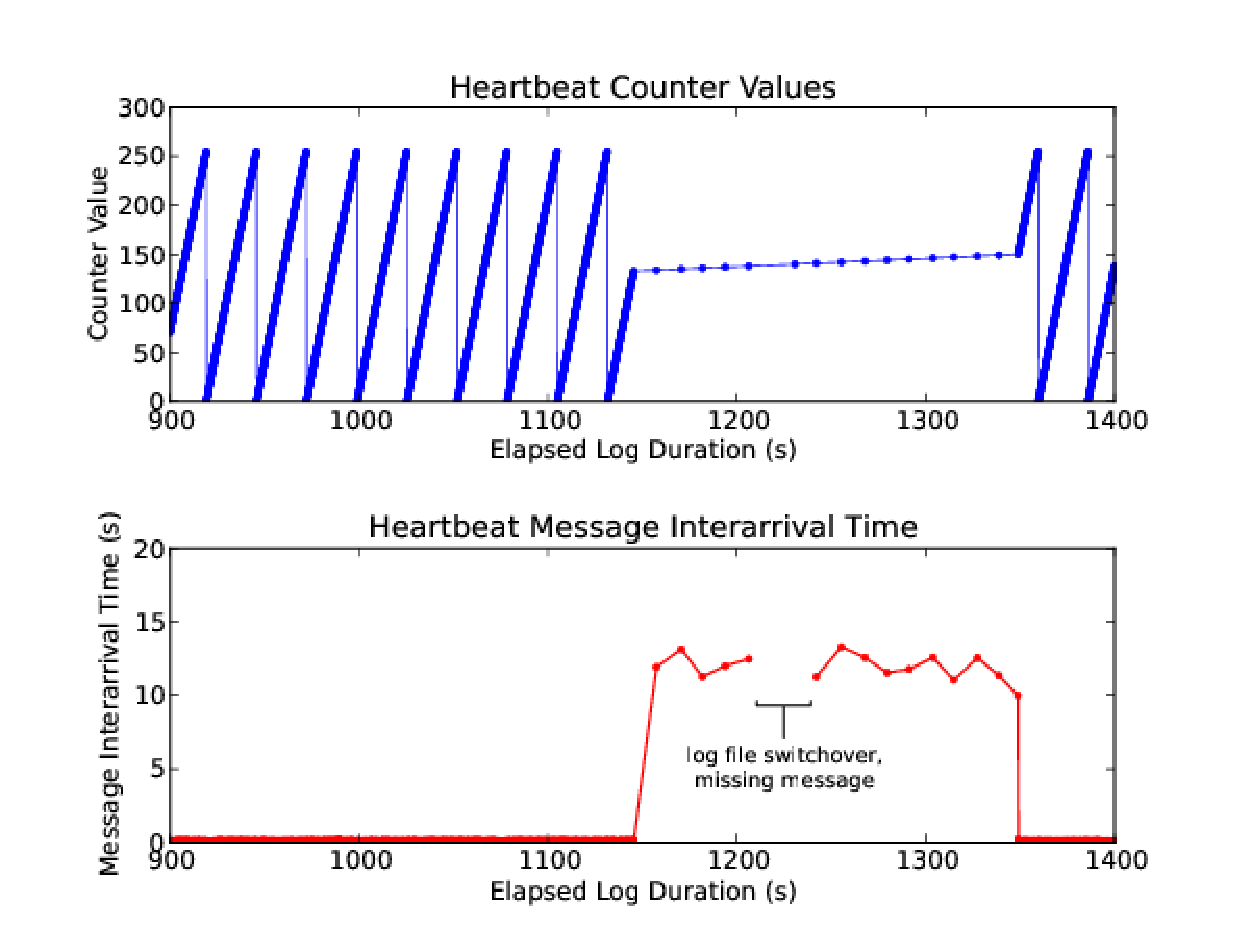
\includegraphics[width=4.5in]{img/hb1}
		\caption{Heartbeat counter values over time}
		\label{fig:hb_arrival}
\end{figure}

% bad status
The second violation is on-time heartbeat status message but the heartbeat status field is 0. 
We do not know from the available documentation whether a bad status in an on-time message with a good counter is valid or not. So without more information we cannot tell whether these violations are false positives or not. This is worthy of further investigation.

% bad counter
The last type of violation is a bad counter. 
We have defined a good counter as one which increments by one every message up to its maximum (255 in this case) before wrapping back to zero.
Every consecutive heartbeat status message must have an incremented heartbeat counter or a violation will be triggered. Figure \ref{fig:hb_badcounter} shows the counter value history for one of the traces with a heartbeat violation caused by a bad counter value.
%
%@EDIT describe robustness testing, define these false positives like the talk?
Further inspection of this violation showed that the bad counter values were sent by the testing framework rather than the actual system. In this case, the network traffic the monitor is seeing is not real system state but actually it is messages being injected by the testing framework. This is not a real violation (since the violating state is not the actual system state), and so we consider this a false positive violation.


\begin{figure}
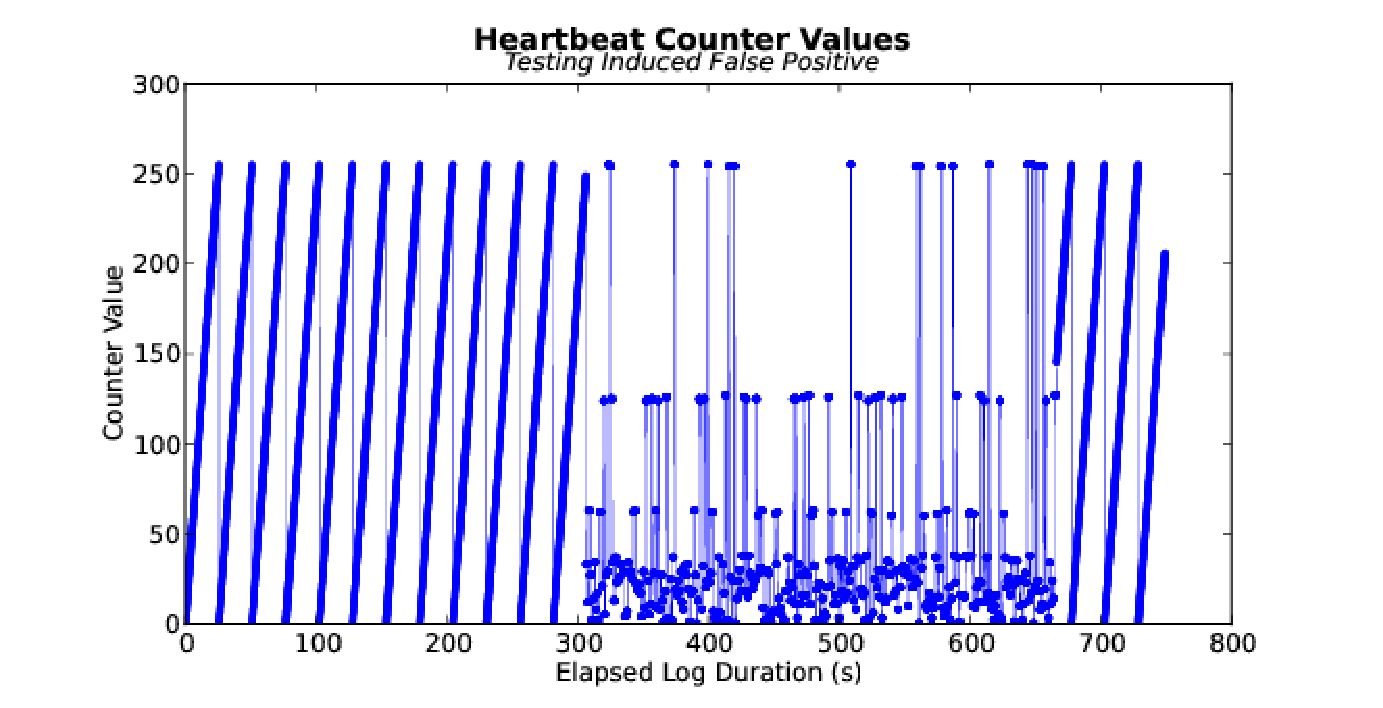
\includegraphics[width=4.5in]{img/hb2}
\caption{Bad heartbeat counter values \label{fig:hb_badcounter}}
\end{figure}

The monitor also reported violations of the legal transition rules, but these, similar to the heartbeat counter violation, also turned out to be false positives triggered by message injections by the robustness testing harness. Since the monitor checks network state, if we perform testing that directly affects the values seen on the network (such as injection/interception of network messages) we may detect violations which are created by the testing framework rather than the system. 
Information about the test configurations can be used to filter out these types of false positives which arise from test-controlled state.
This type of filtering can be automated if the test information can be input to the monitor, either directly on the network (e.g., adding a message value to injected messages) or through a side-channel (i.e., building a testing-aware monitor).

%%%% Conclusion section

\section{Future Work and Conclusion}
We have developed a runtime monitoring approach for an ARV system.
Instead of instrumention, we passively monitor the system,
generating the system trace from the observed network state.
We have developed an efficient runtime monitoring algorithm, \monitor,
that eagerly checks for violations of properties written in future-bounded
propositional MTL. We have shown the efficiency of \monitor by implementing it
and evaluating it against logs obtained from system testing of the ARV.
\monitor was able to detect violations of several safety requirements in real-time.
Future work includes exploring monitors running in multi-core environment
to provide increased monitoring power as well as further
formalizing the interface mapping (possibly with a domain specific language).



%\def\IEEEbibitemsep{0pt plus .5pt}
\bibliographystyle{splncs03}
% argument is your BibTeX string definitions and bibliography database(s)
\bibliography{./rv2015_bibtex}

\end{document}
